This is about the alphasense CO results.

Two AlphaSense CO sensors were tested against the EPA reference.  The first sensor was 2.5 years old at the time of installation,  which ran for 38 days (from 4/15 to 5/23 2016 with one 40 minute service interruption).  The second sensor was 2 months old at the time of installation, and ran for 21 days (from 5/23 - 6/13 2016).  Our first test gave 55,589 minute-resolution samples to compare, our second test gave 30,150 samples.

Age is an important distinction between the two sensors, which makes this an interesting comparison.  Additionally, while the first CO sensor was only calibrated for CO measurement.

\subsection{Pre-processing}

Talk about process for taking raw aux/working electrodes and making the basic calibration data.

Old sensor, raw data with simple calibration based on datasheet.


\begin{figure}[htb]
 	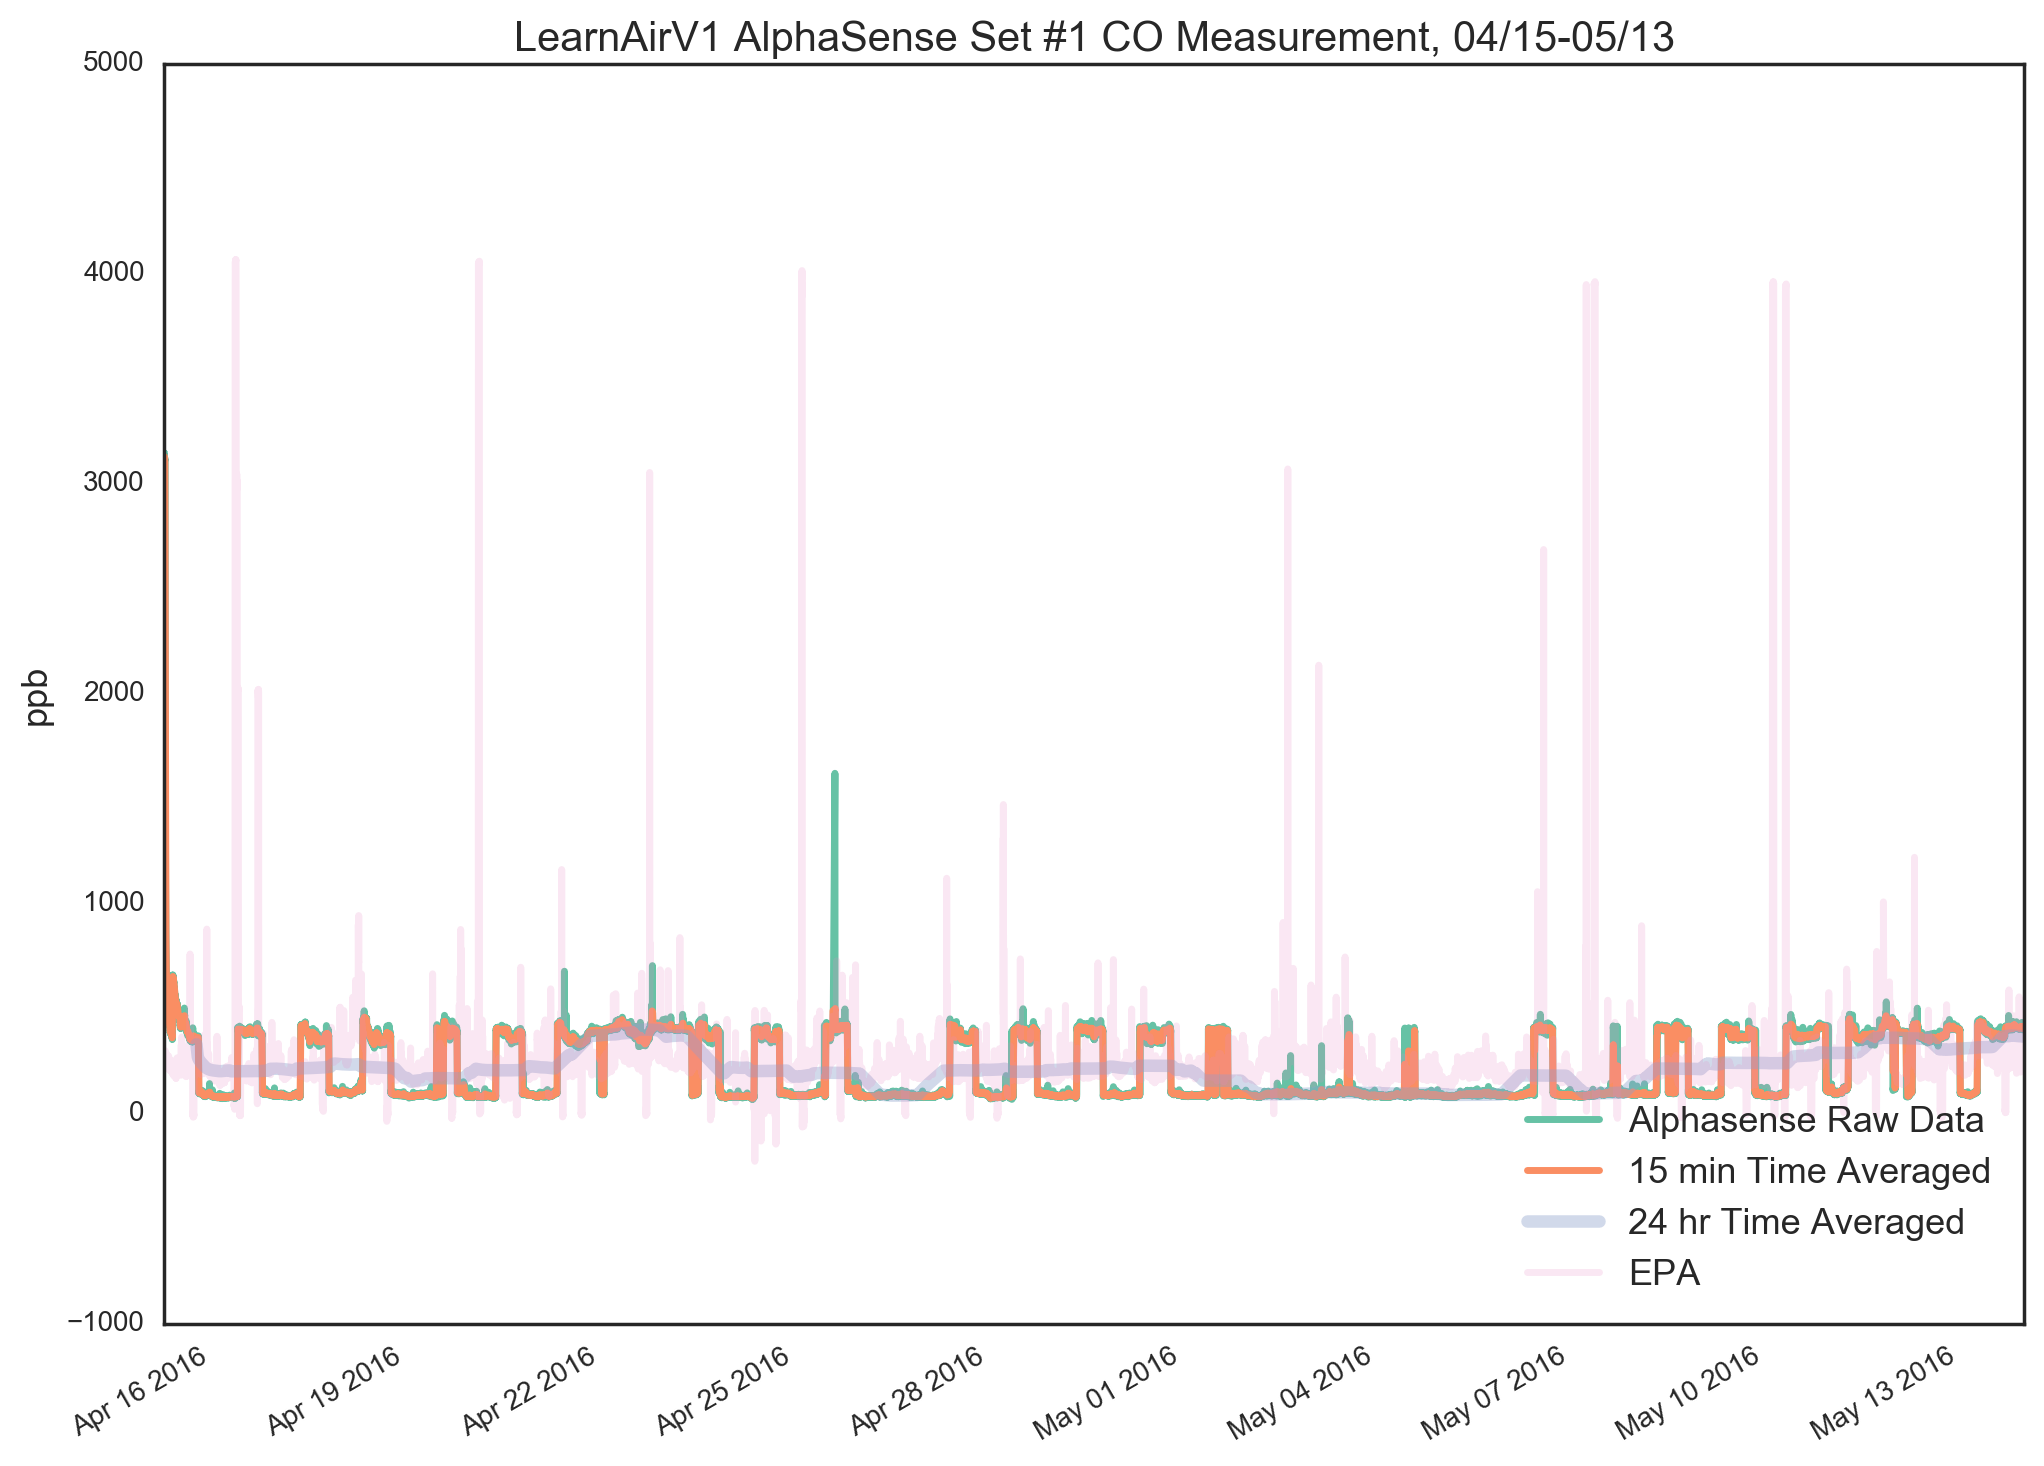
\includegraphics[width=\textwidth]{figs/as_co_raw}               
 	 \caption{AlphaSense CO Sensor #1 Raw Data}
  	\label{fig:as_co_raw}
\end{figure}


\begin{figure}[htb]
 	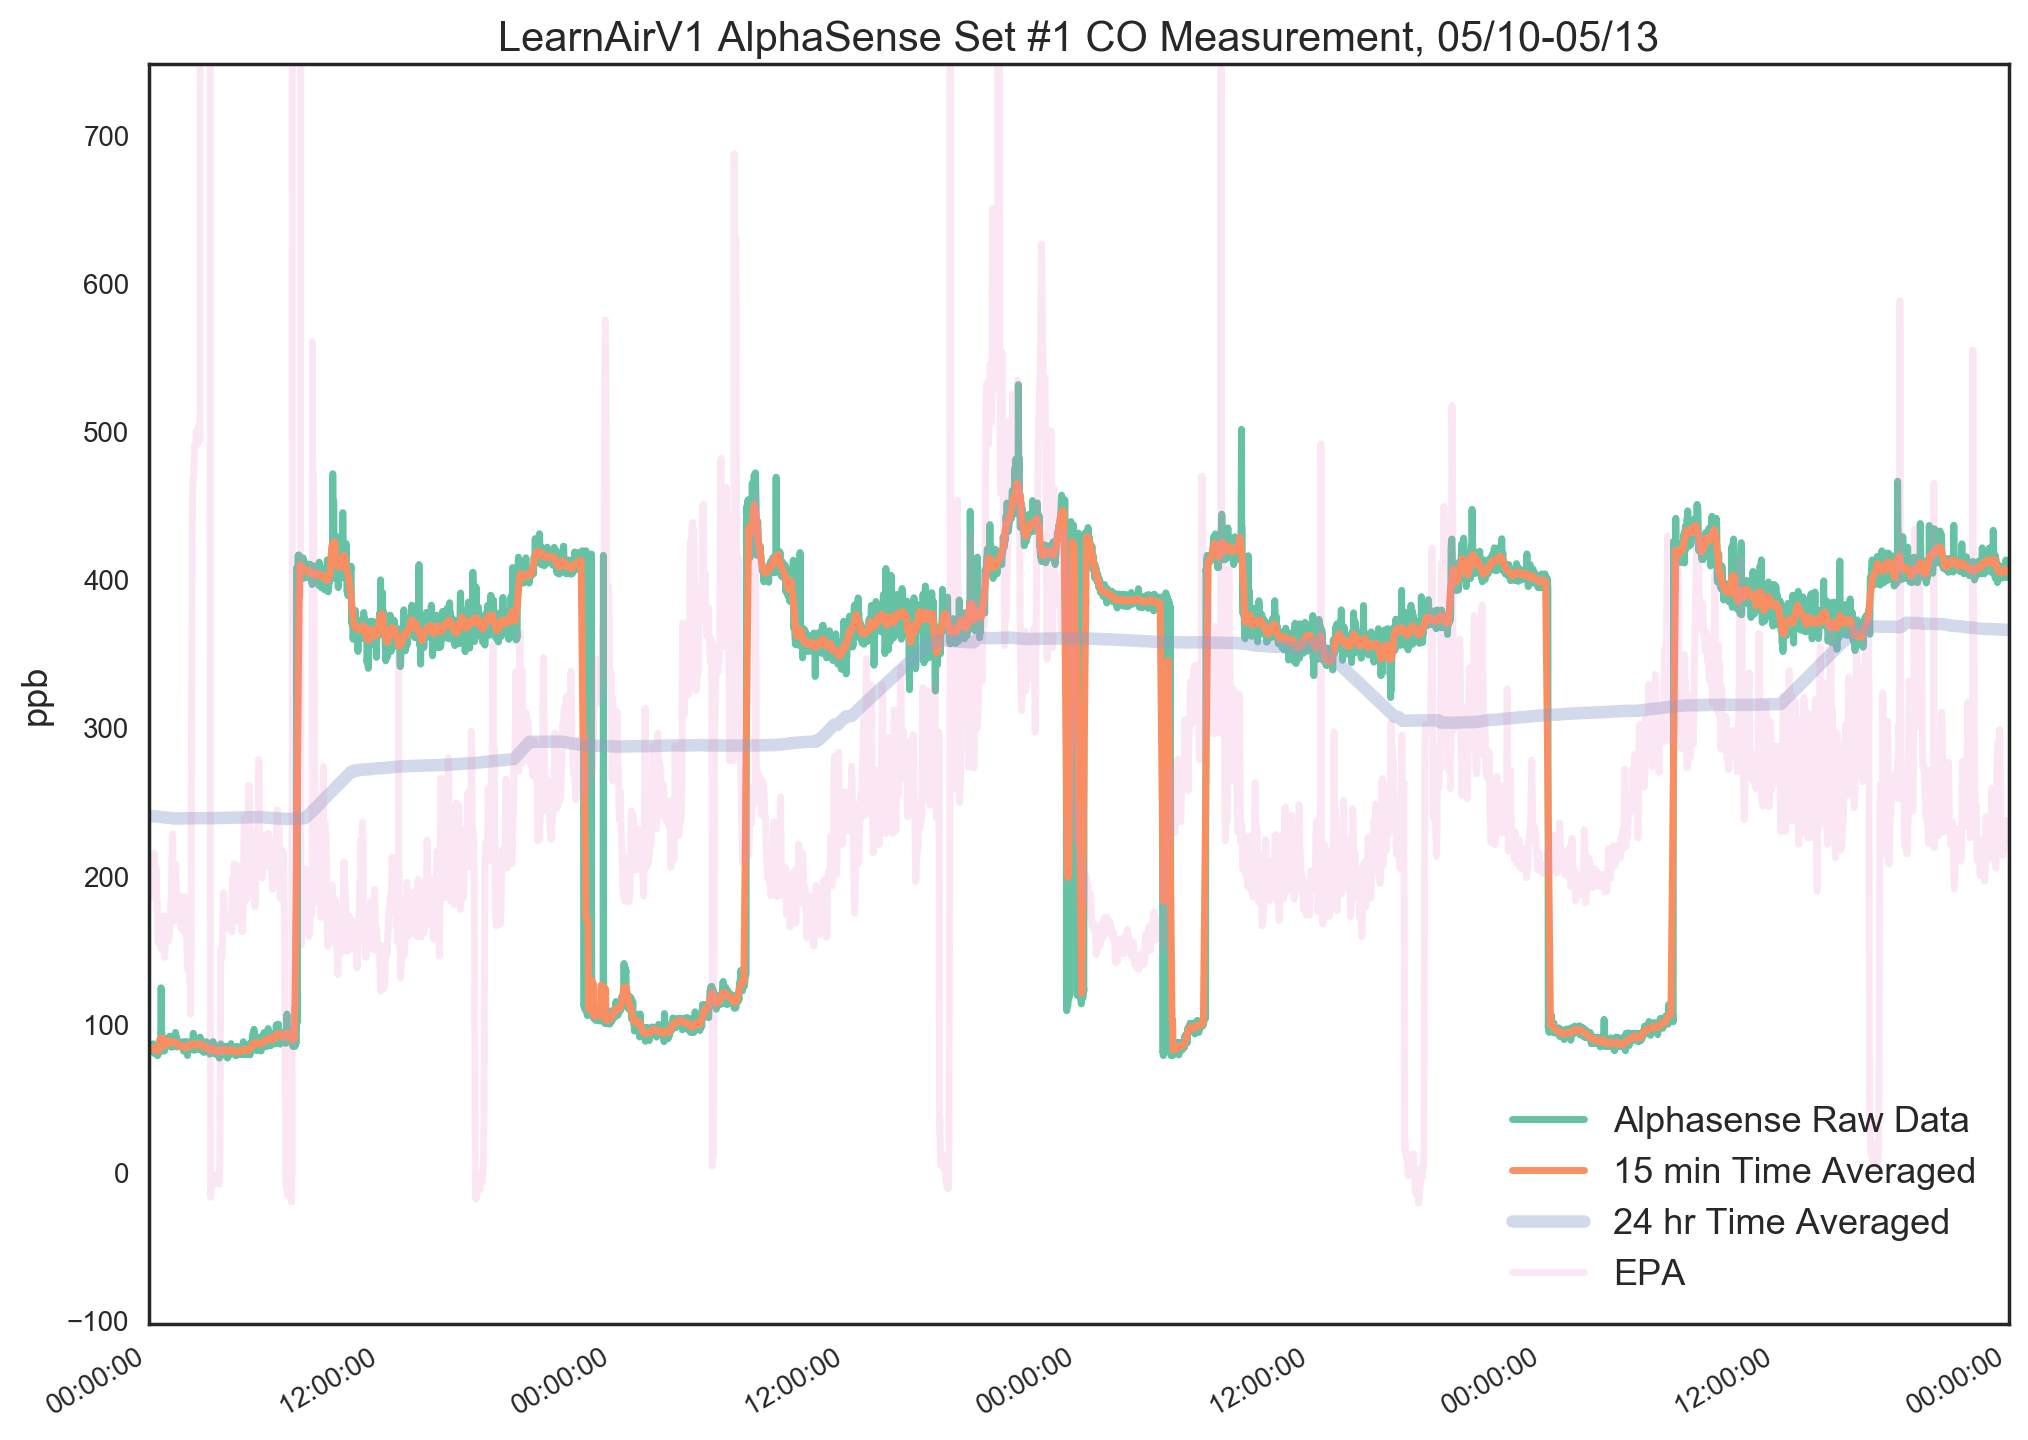
\includegraphics[width=\textwidth]{figs/as_co_raw_zoomed}               
 	 \caption{AlphaSense CO Sensor #1 Raw Data Zoomed}
  	\label{fig:as_co_raw_zoomed}
\end{figure}



\begin{figure}[htb]
 	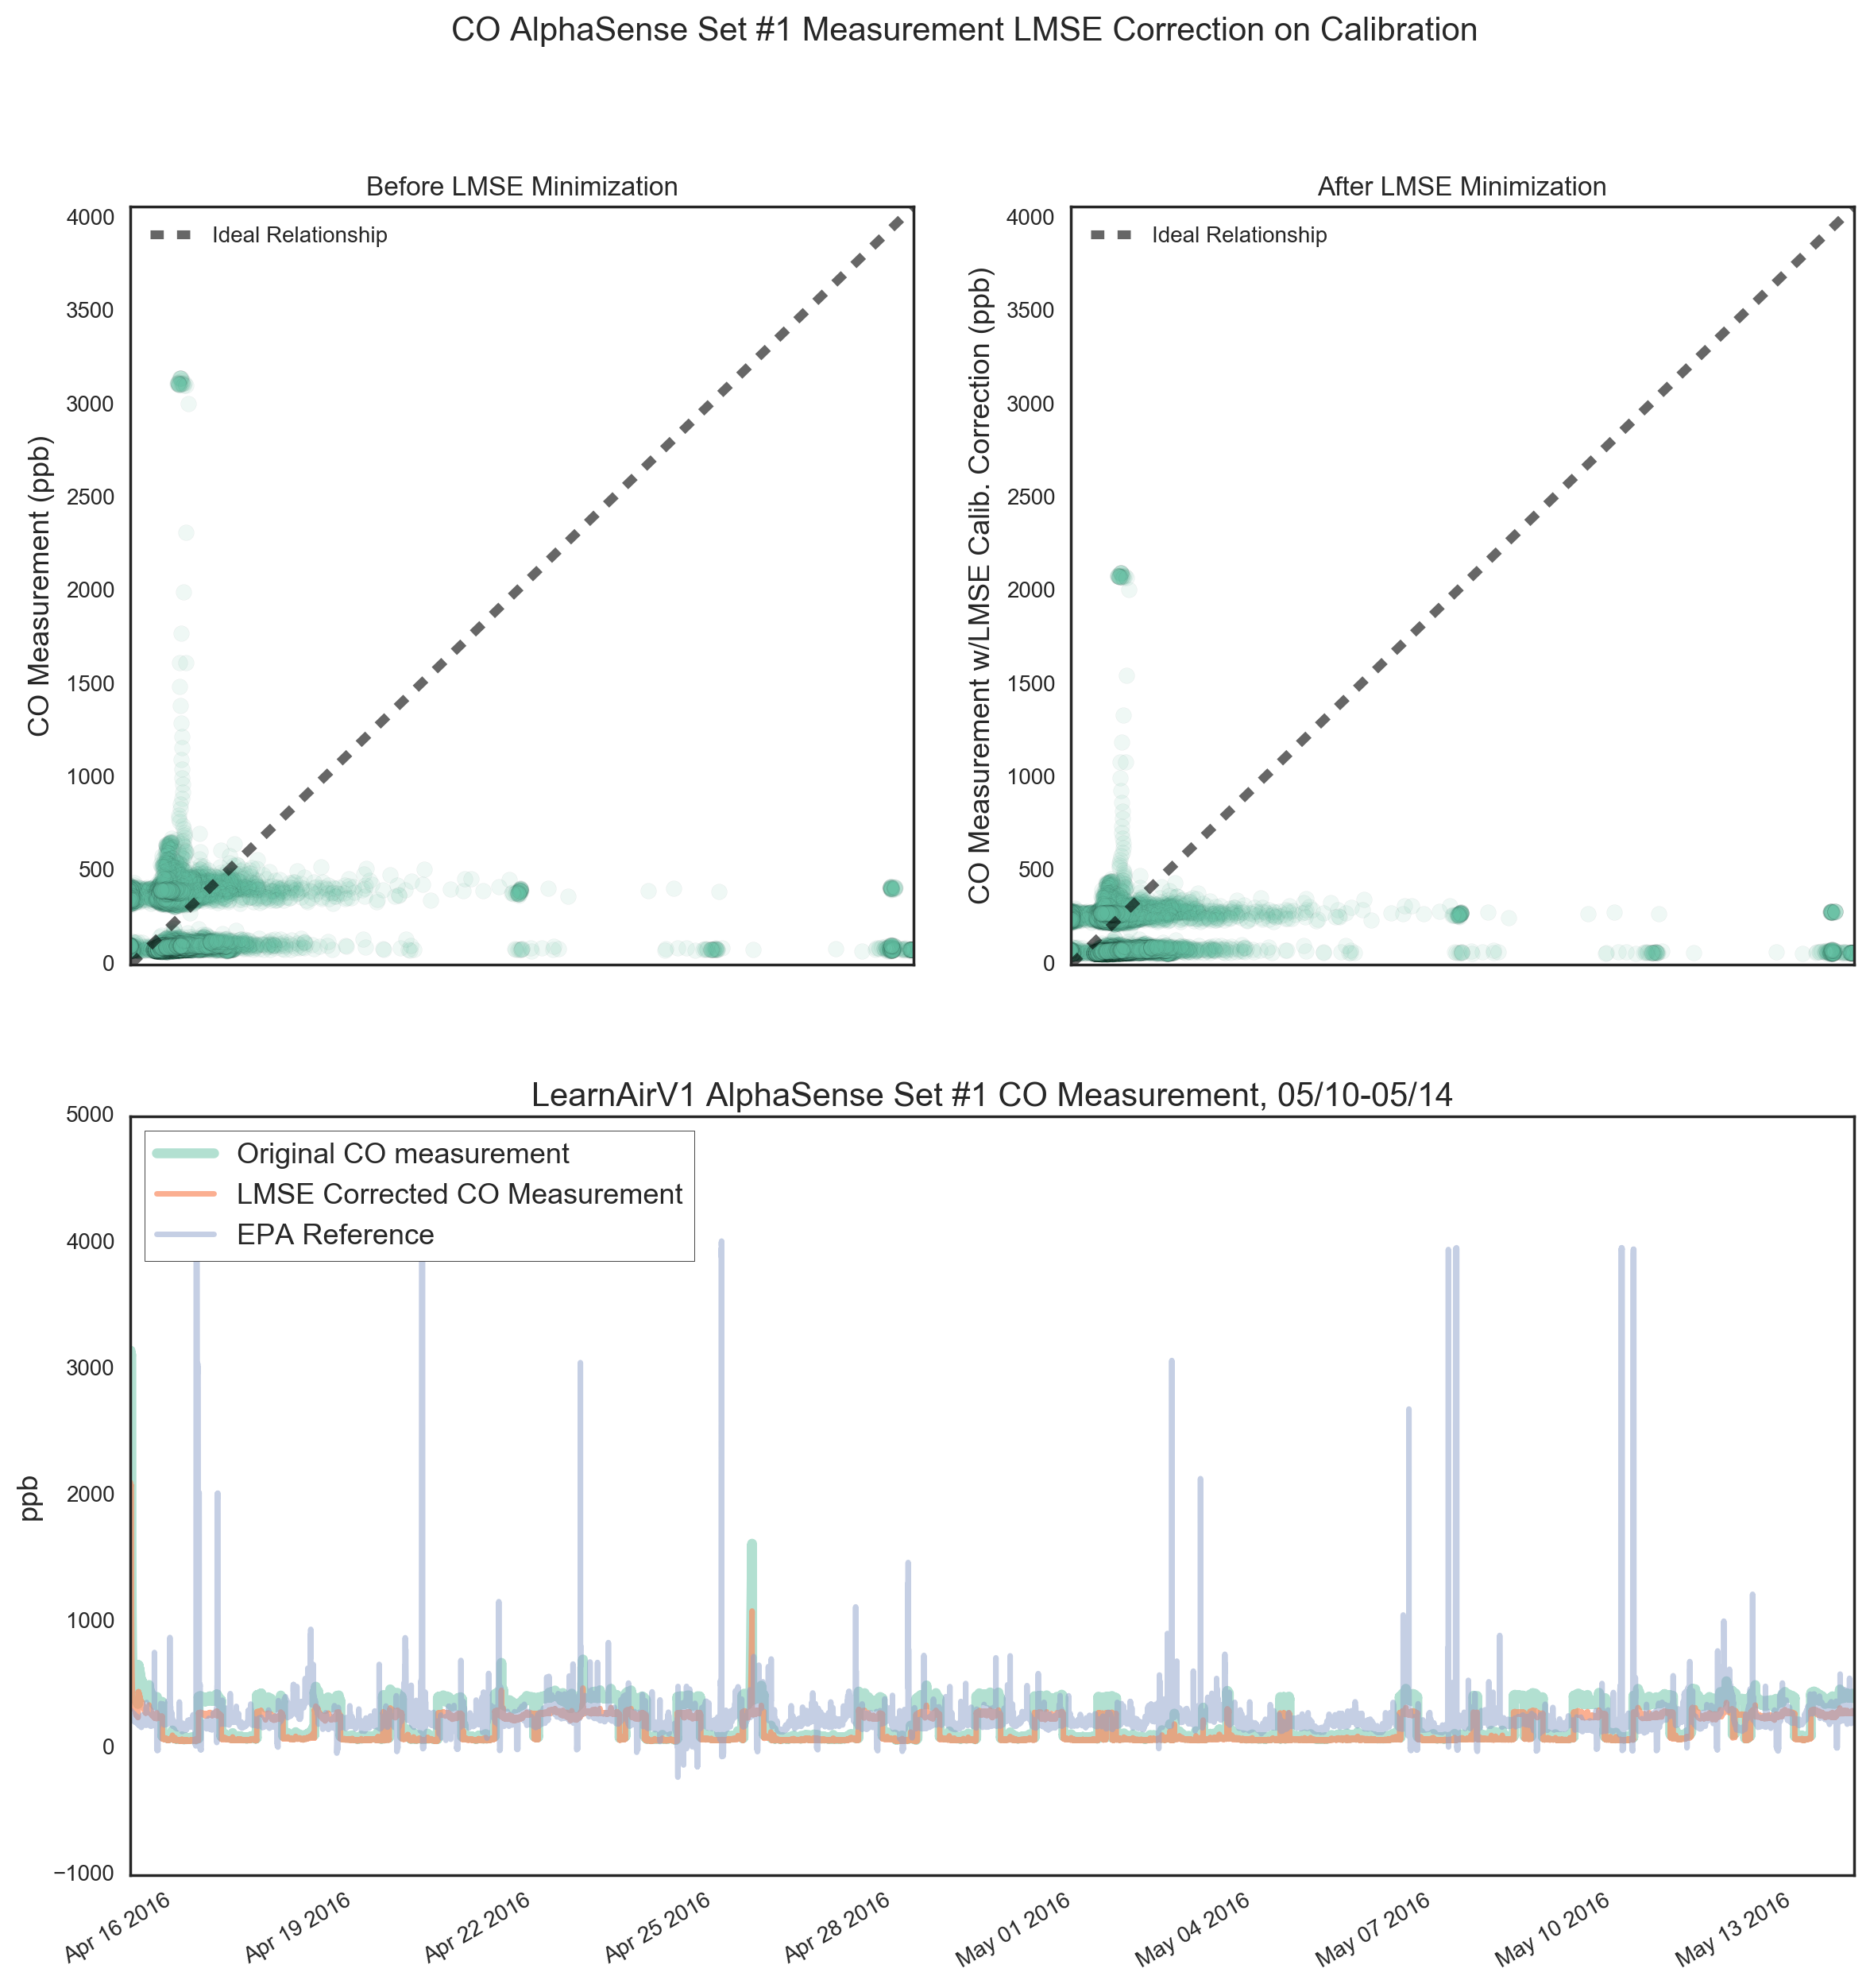
\includegraphics[width=\textwidth]{figs/as1_co_lmse}               
 	 \caption{AlphaSense CO Sensor #1 after LMSE Calibration}
  	\label{fig:as1_co_lmse}
\end{figure}

\begin{figure}[htb]
 	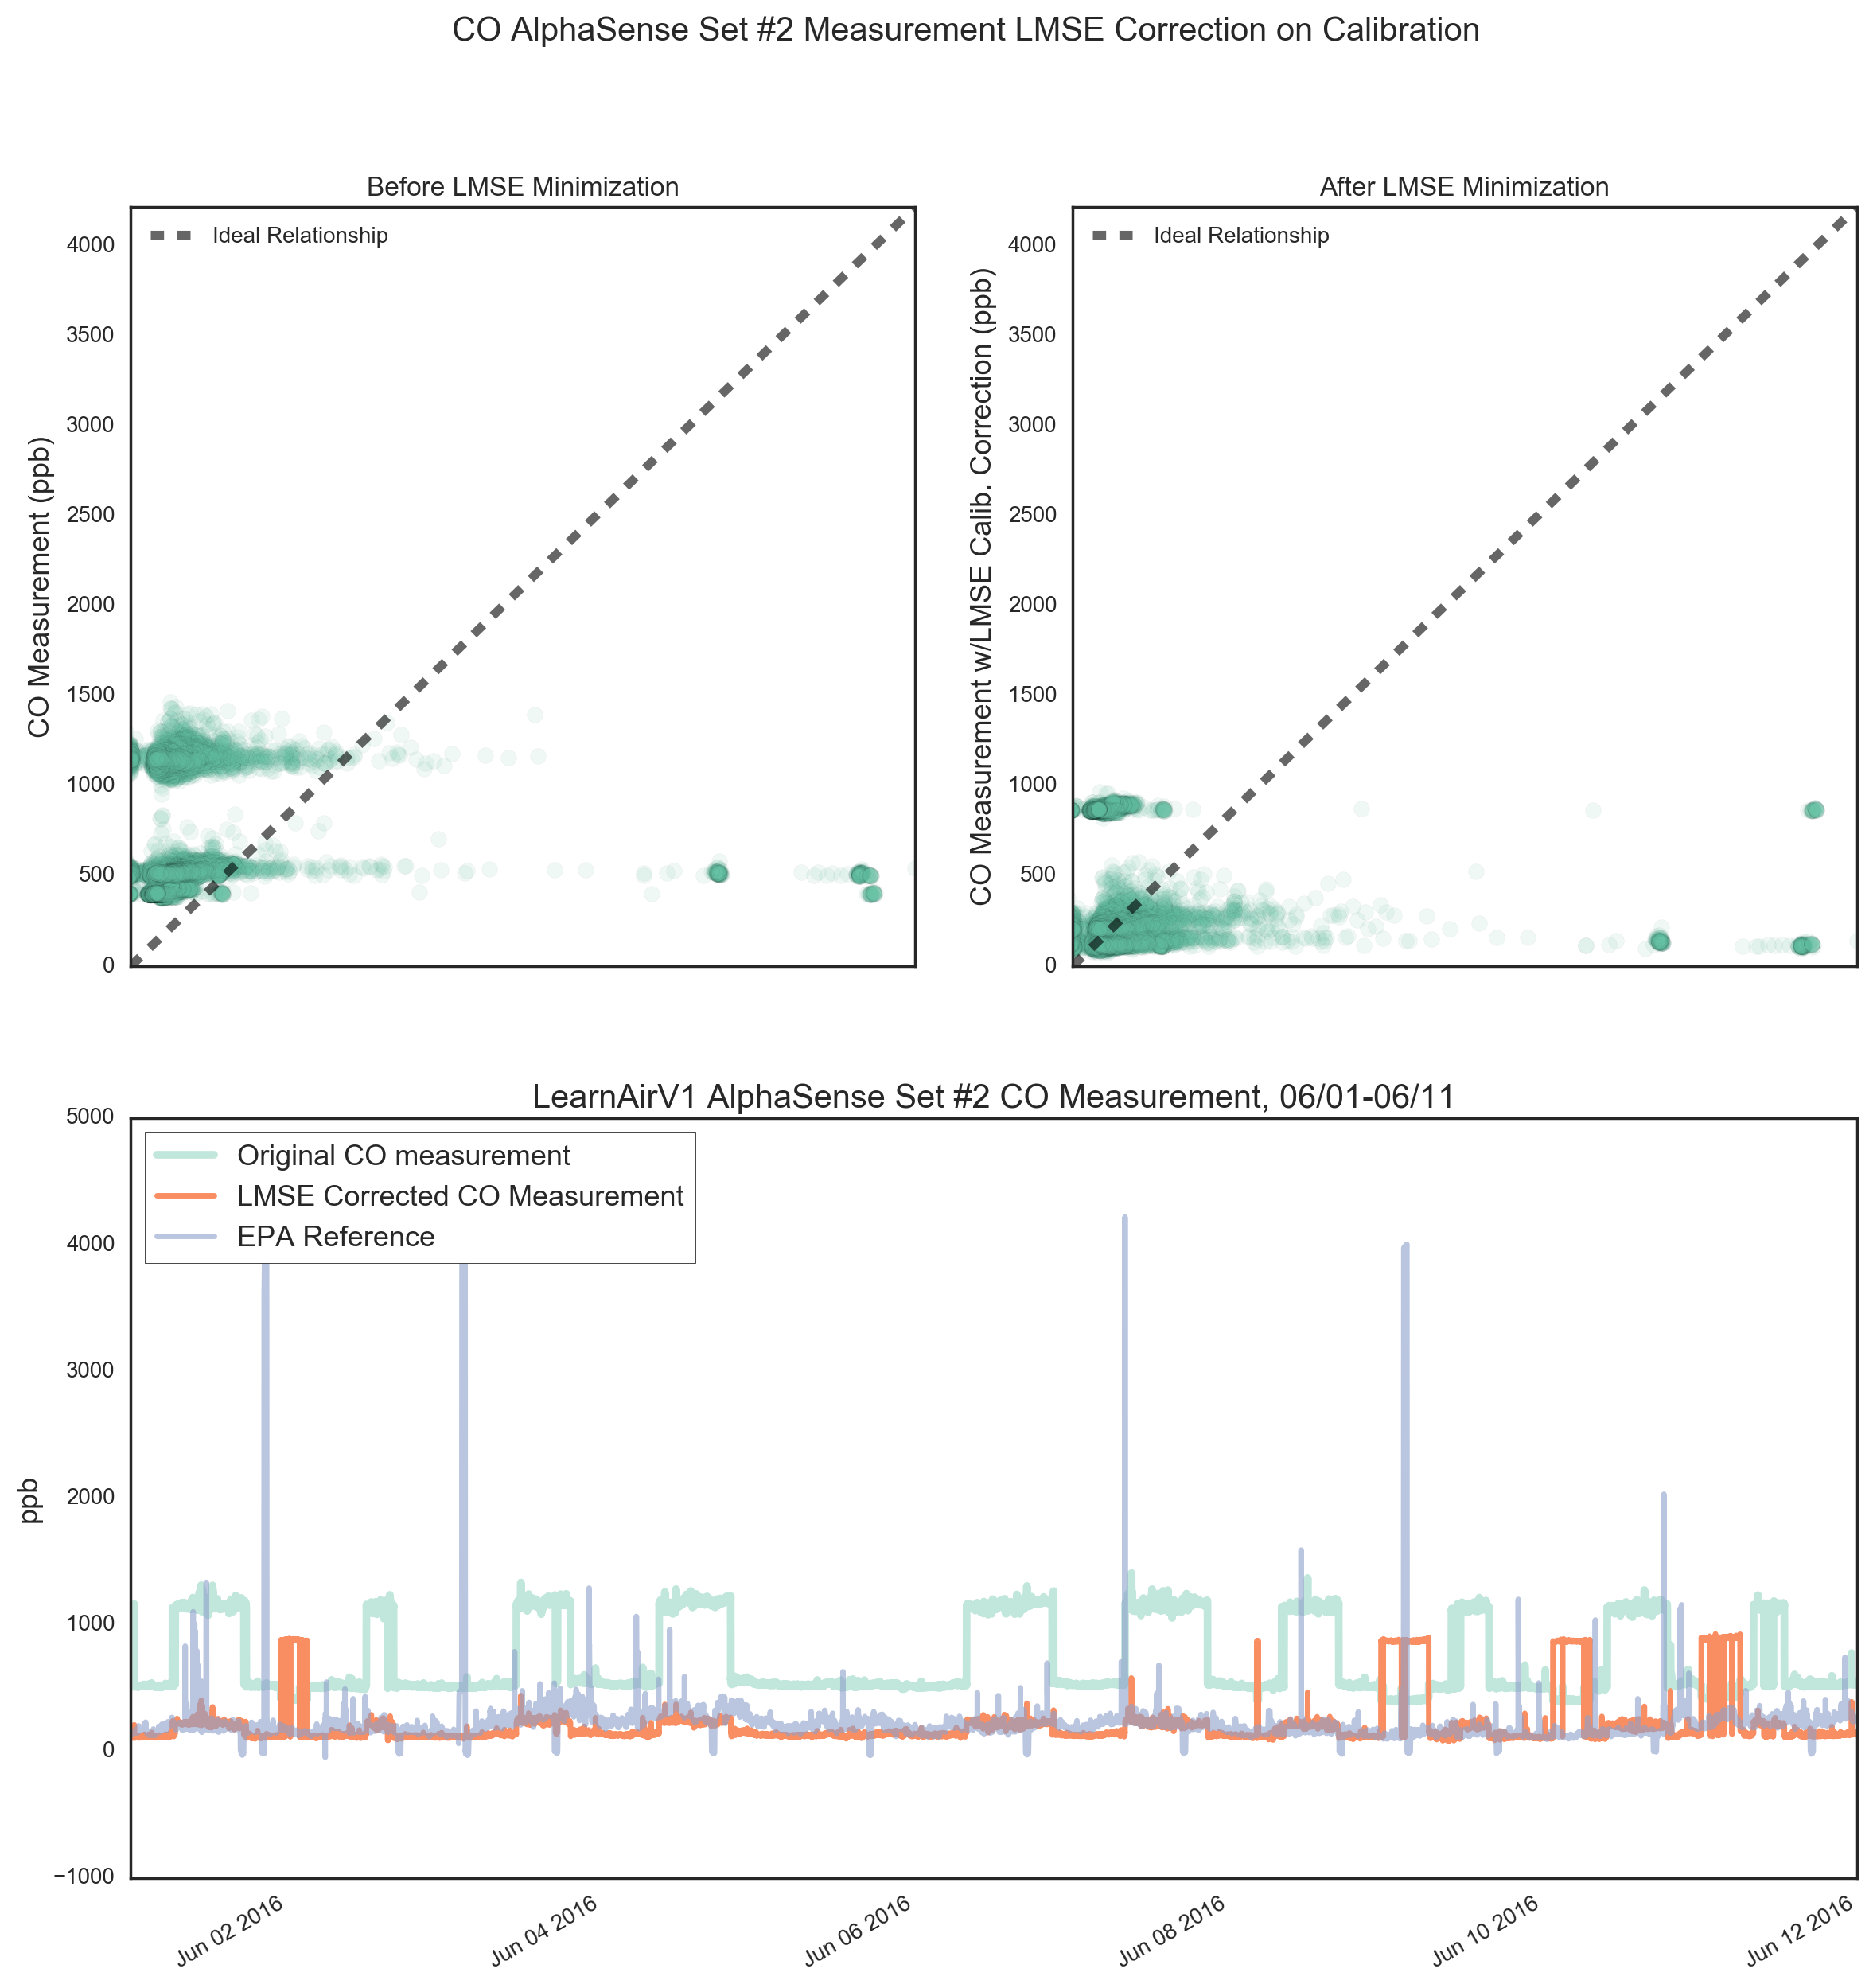
\includegraphics[width=\textwidth]{figs/as2_co_lmse}               
 	 \caption{AlphaSense CO Sensor #2 after LMSE Calibration}
  	\label{fig:as2_co_lmse}
\end{figure}







\subsection{Machine Learning}


\begin{figure}[htb]
 	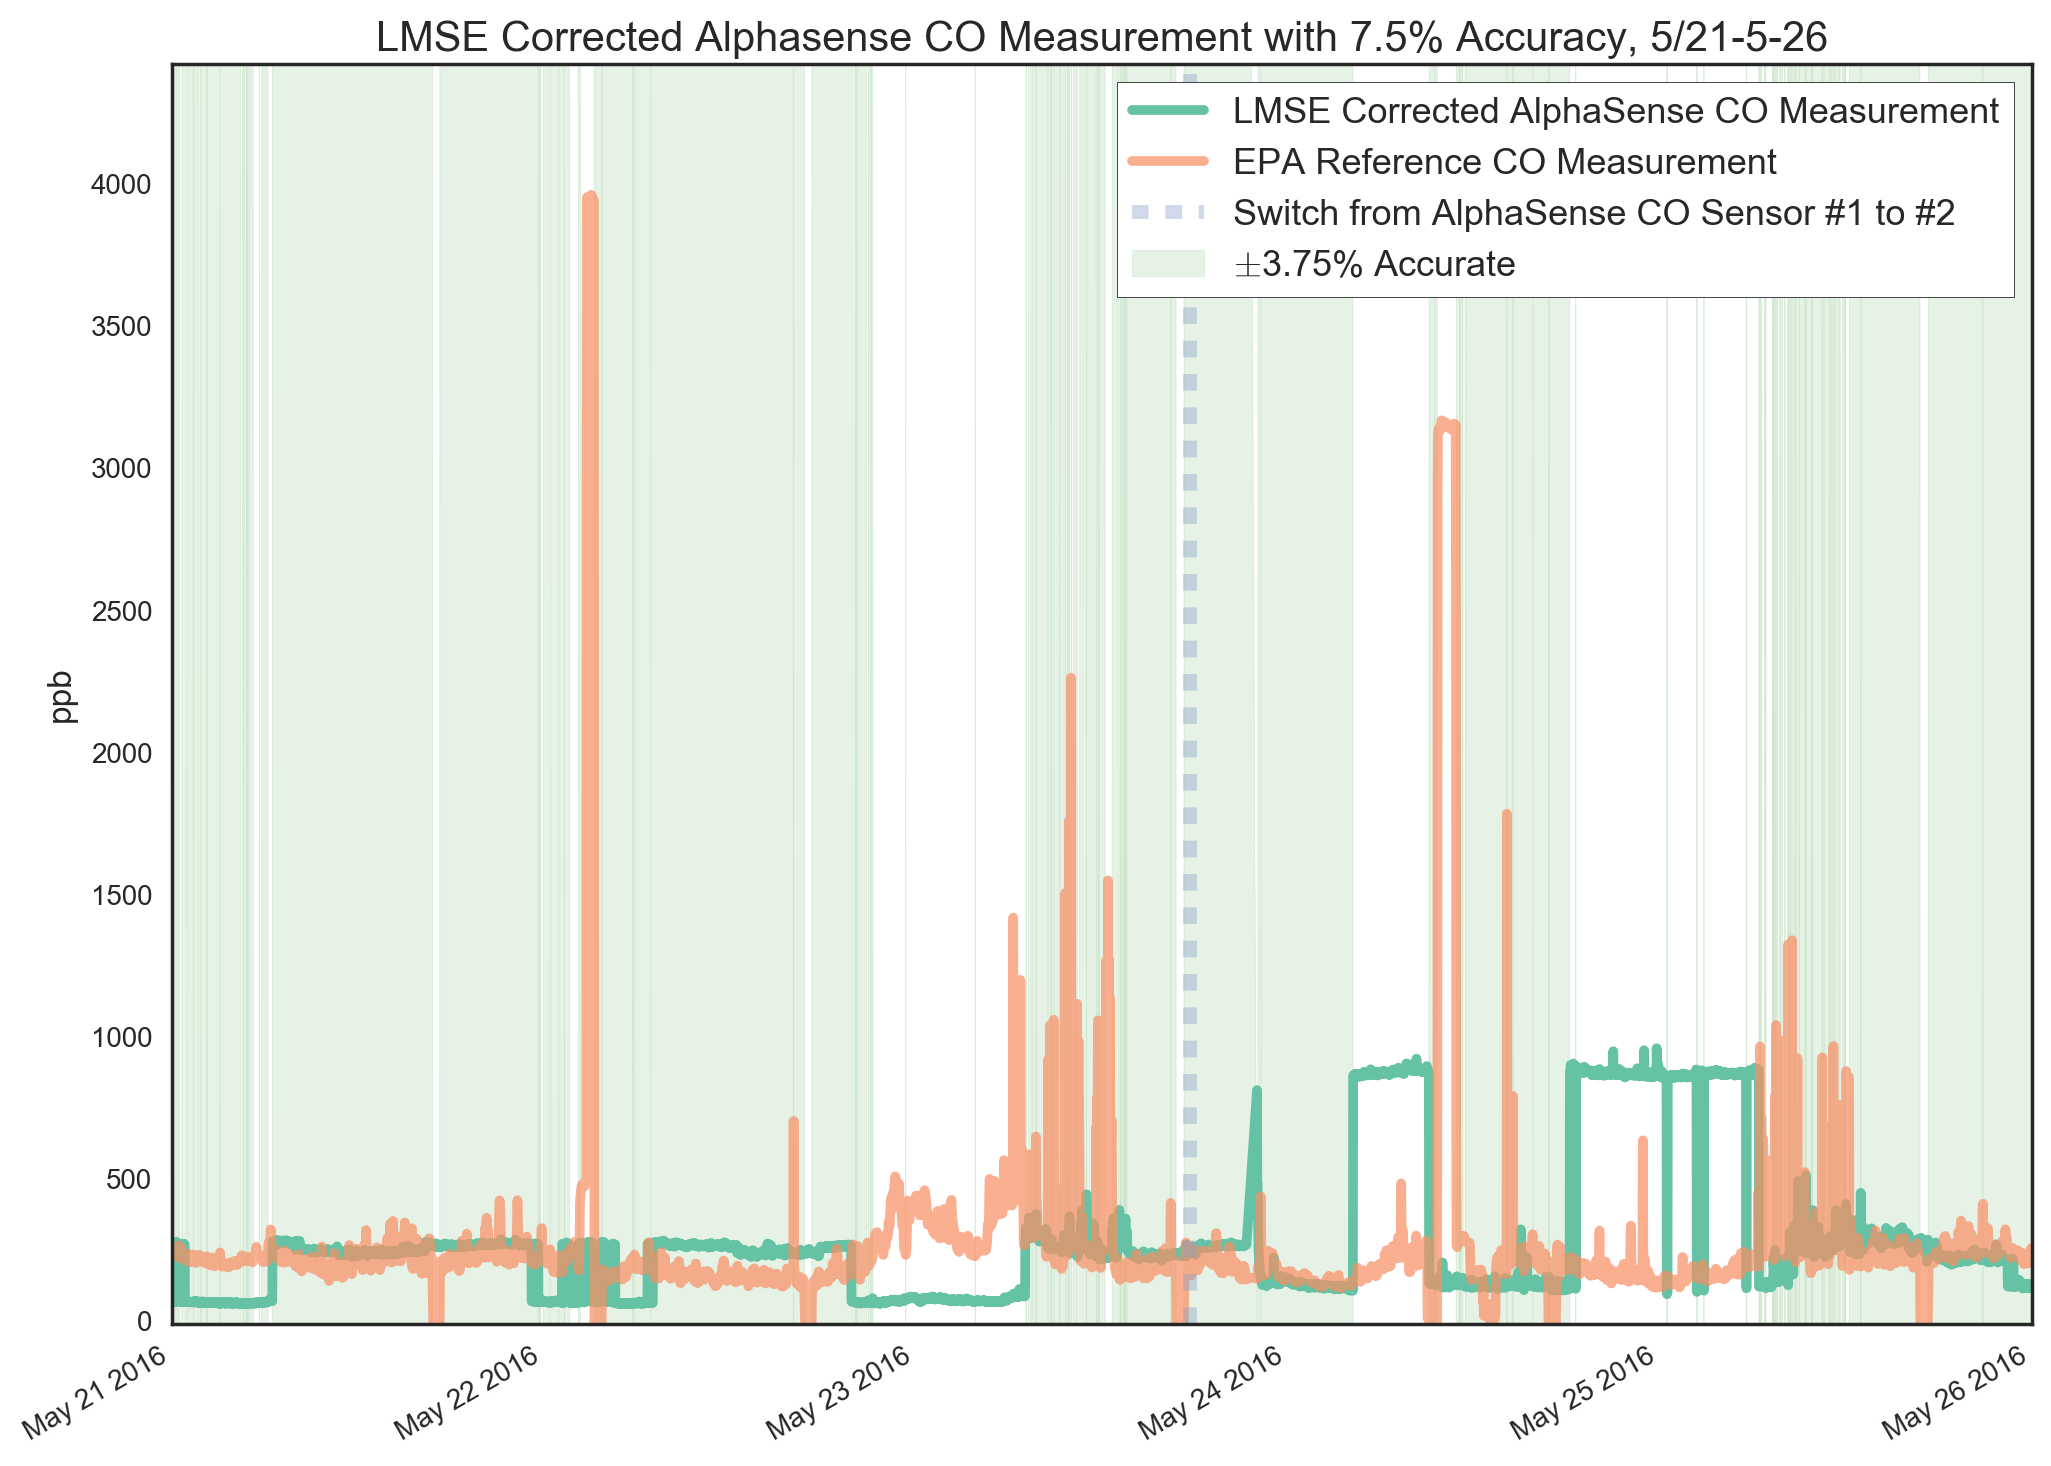
\includegraphics[width=\textwidth]{figs/as_co_with_7p5_accuracy_zoomed}               
 	 \caption{AlphaSense CO Sensor #1 and #2 with 7.5\% Accuracy Threshold}
  	\label{fig:as_co_with_7p5_accuracy_zoomed}
\end{figure}

\begin{figure}[htb]
 	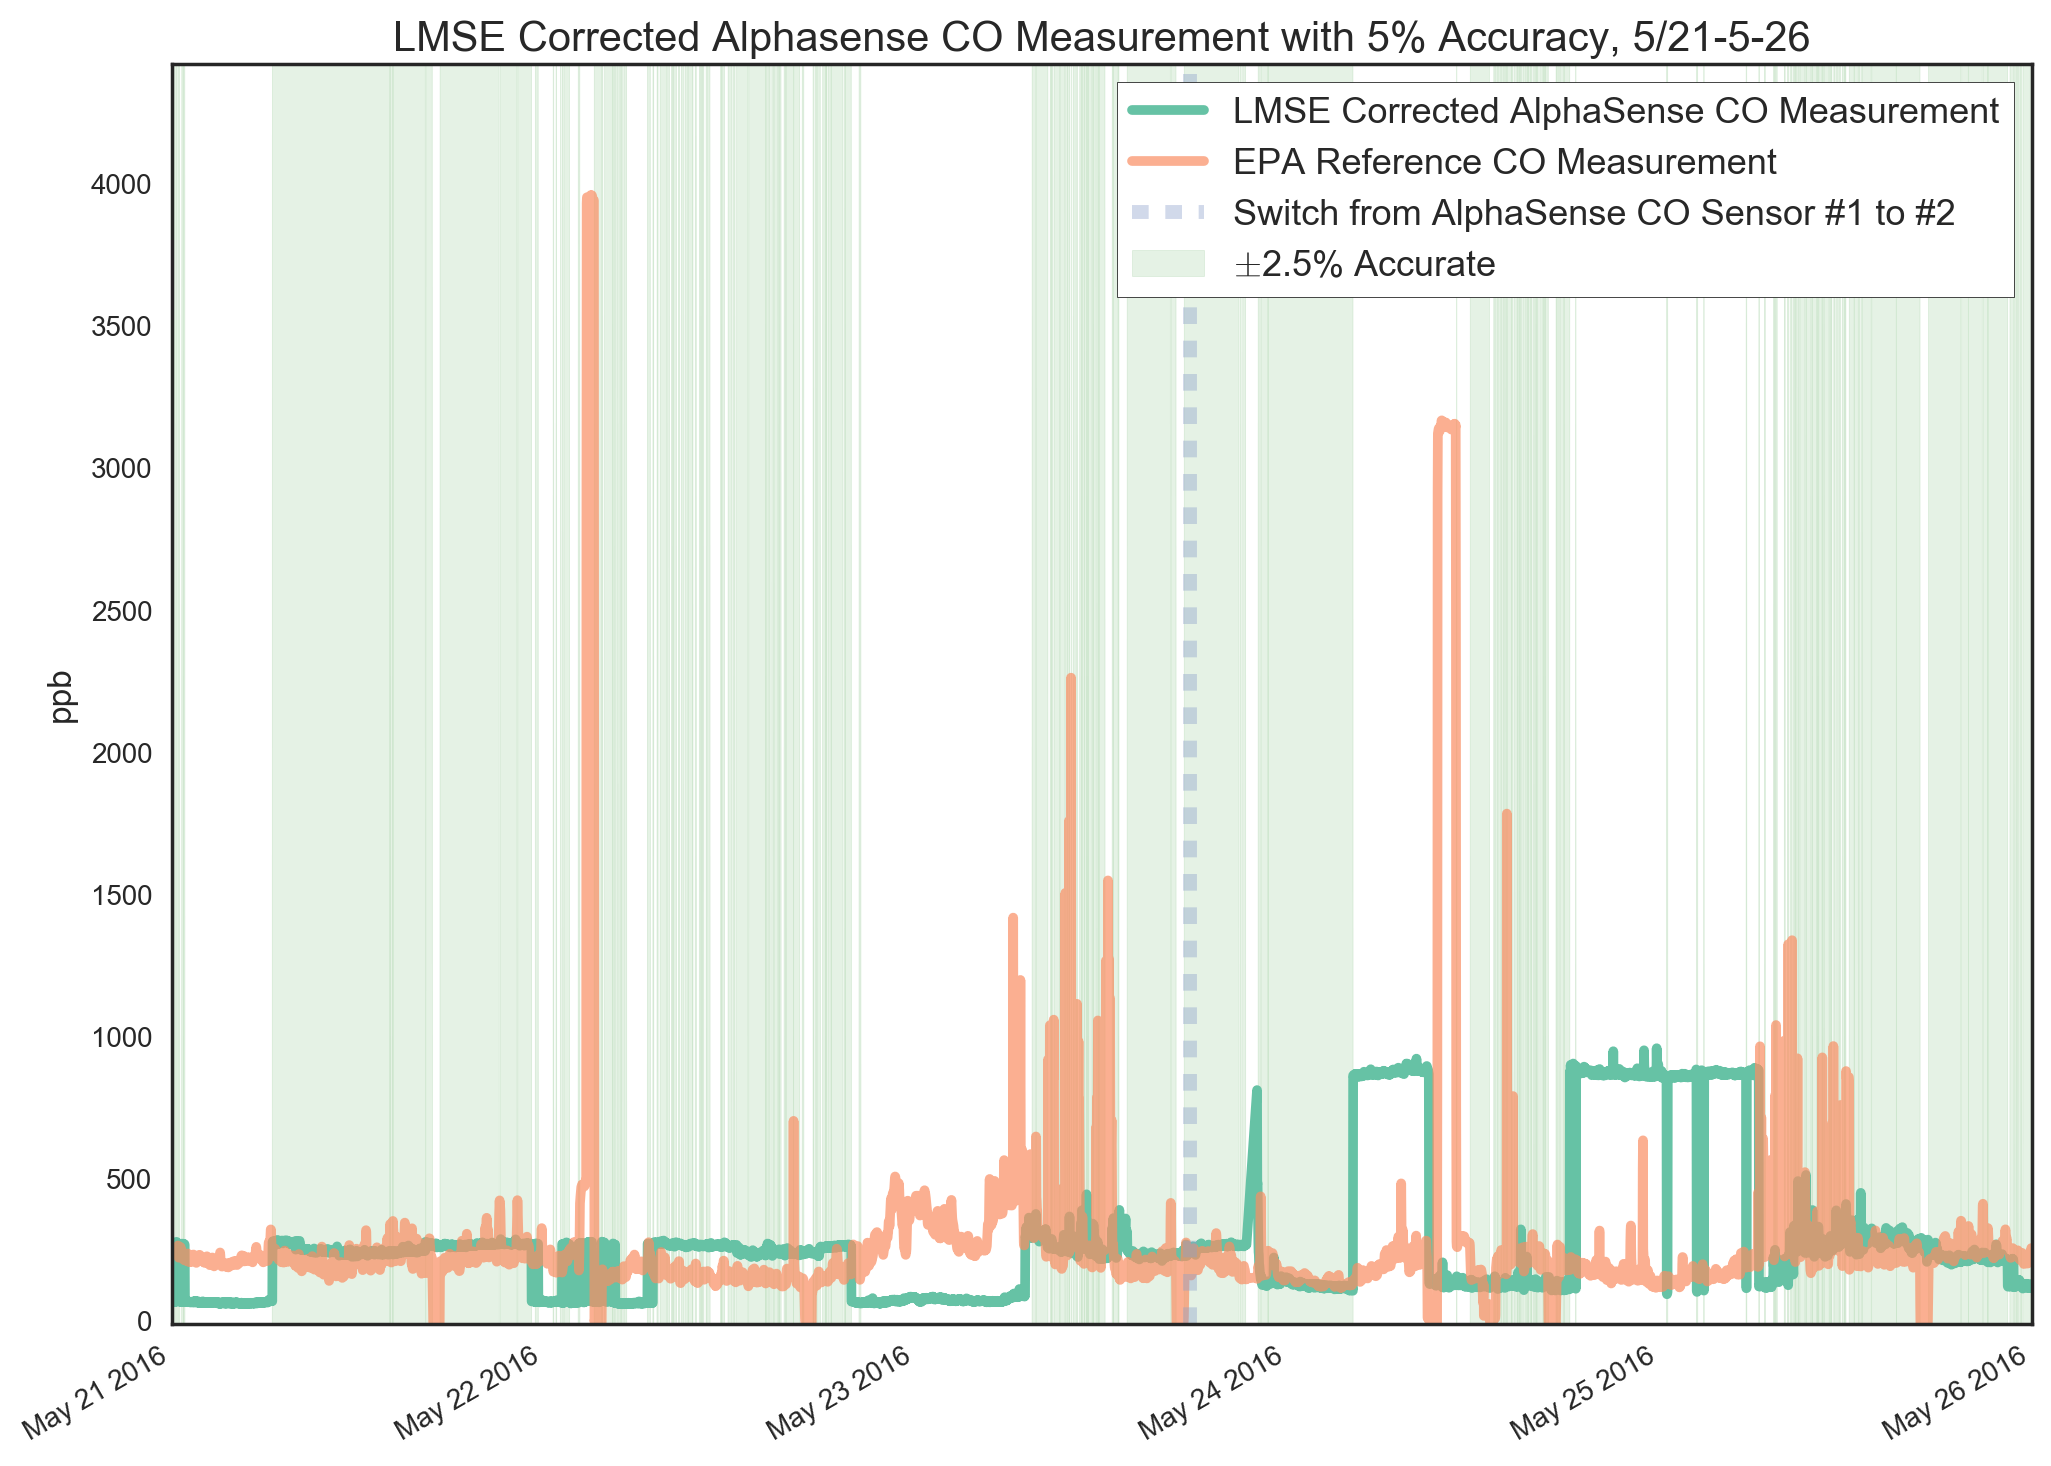
\includegraphics[width=\textwidth]{figs/as_co_with_5_accuracy_zoomed}               
 	 \caption{AlphaSense CO Sensor #1 and #2 with 5\% Accuracy Threshold}
  	\label{fig:as_co_with_5_accuracy_zoomed}
\end{figure}






parameters = {'C':[0.001, 0.1, 10, 1000], 'penalty':('L1', 'L2') }

===== best ROC\_AUC score 0.894883095983

===== best params {'penalty': 'L1', 'C': 1000}



\begin{table}[H]
\centering
\begin{tabular}{|c|c|c|c|c|}
\toprule
\multicolumn{5}{|c|}{Error Rates for CO Sensor #1 with Logistic Regression} \\
&\multicolumn{2}{|c|}{all features} & \multicolumn{2}{|c|}{top 15 features} \\
&shuffled & chunked & shuffled & chunked \\
avg & 0.18 & 0.21 & 0.20 & 0.20 \\
min & 0.17 & 0.17 & 0.19 & 0.12 \\
max & 0.18 & 0.28 & 0.20 & 0.28 \\
\bottomrule
\end{tabular}
\label{tab:as1_co_error_rates}
\caption{Error Rates for Predicting CO Sensor #1 Accuracy with Logistic Regression}
\end{table}



\begin{table}[H]
\centering
\offinterlineskip
\hspace*{-5cm}\raisebox{-3.5cm}[0pt][0pt]{\rotatebox[origin=c]{90}{\parbox[c][0pt][c]{3cm}{\textbf{Actual Values}\\[20pt]}}}\par
\hspace*{1cm}\MyHBox[\dimexpr5.1cm+6\fboxsep\relax]{Predicted Values}\par
\hspace*{1cm}\MyHBox{0}\MyHBox{1}\par
\MyTBox{0}{4751.0}{943.0}
\MyTBox{1}{1023.4}{4400.4}
}
\label{tab:as1_co_confusion}
\caption{Average AlphaSense CO Sensor #1 Confusion Matrix w/Shuffled K-Fold}
\end{table}


\begin{figure}[htb]
 	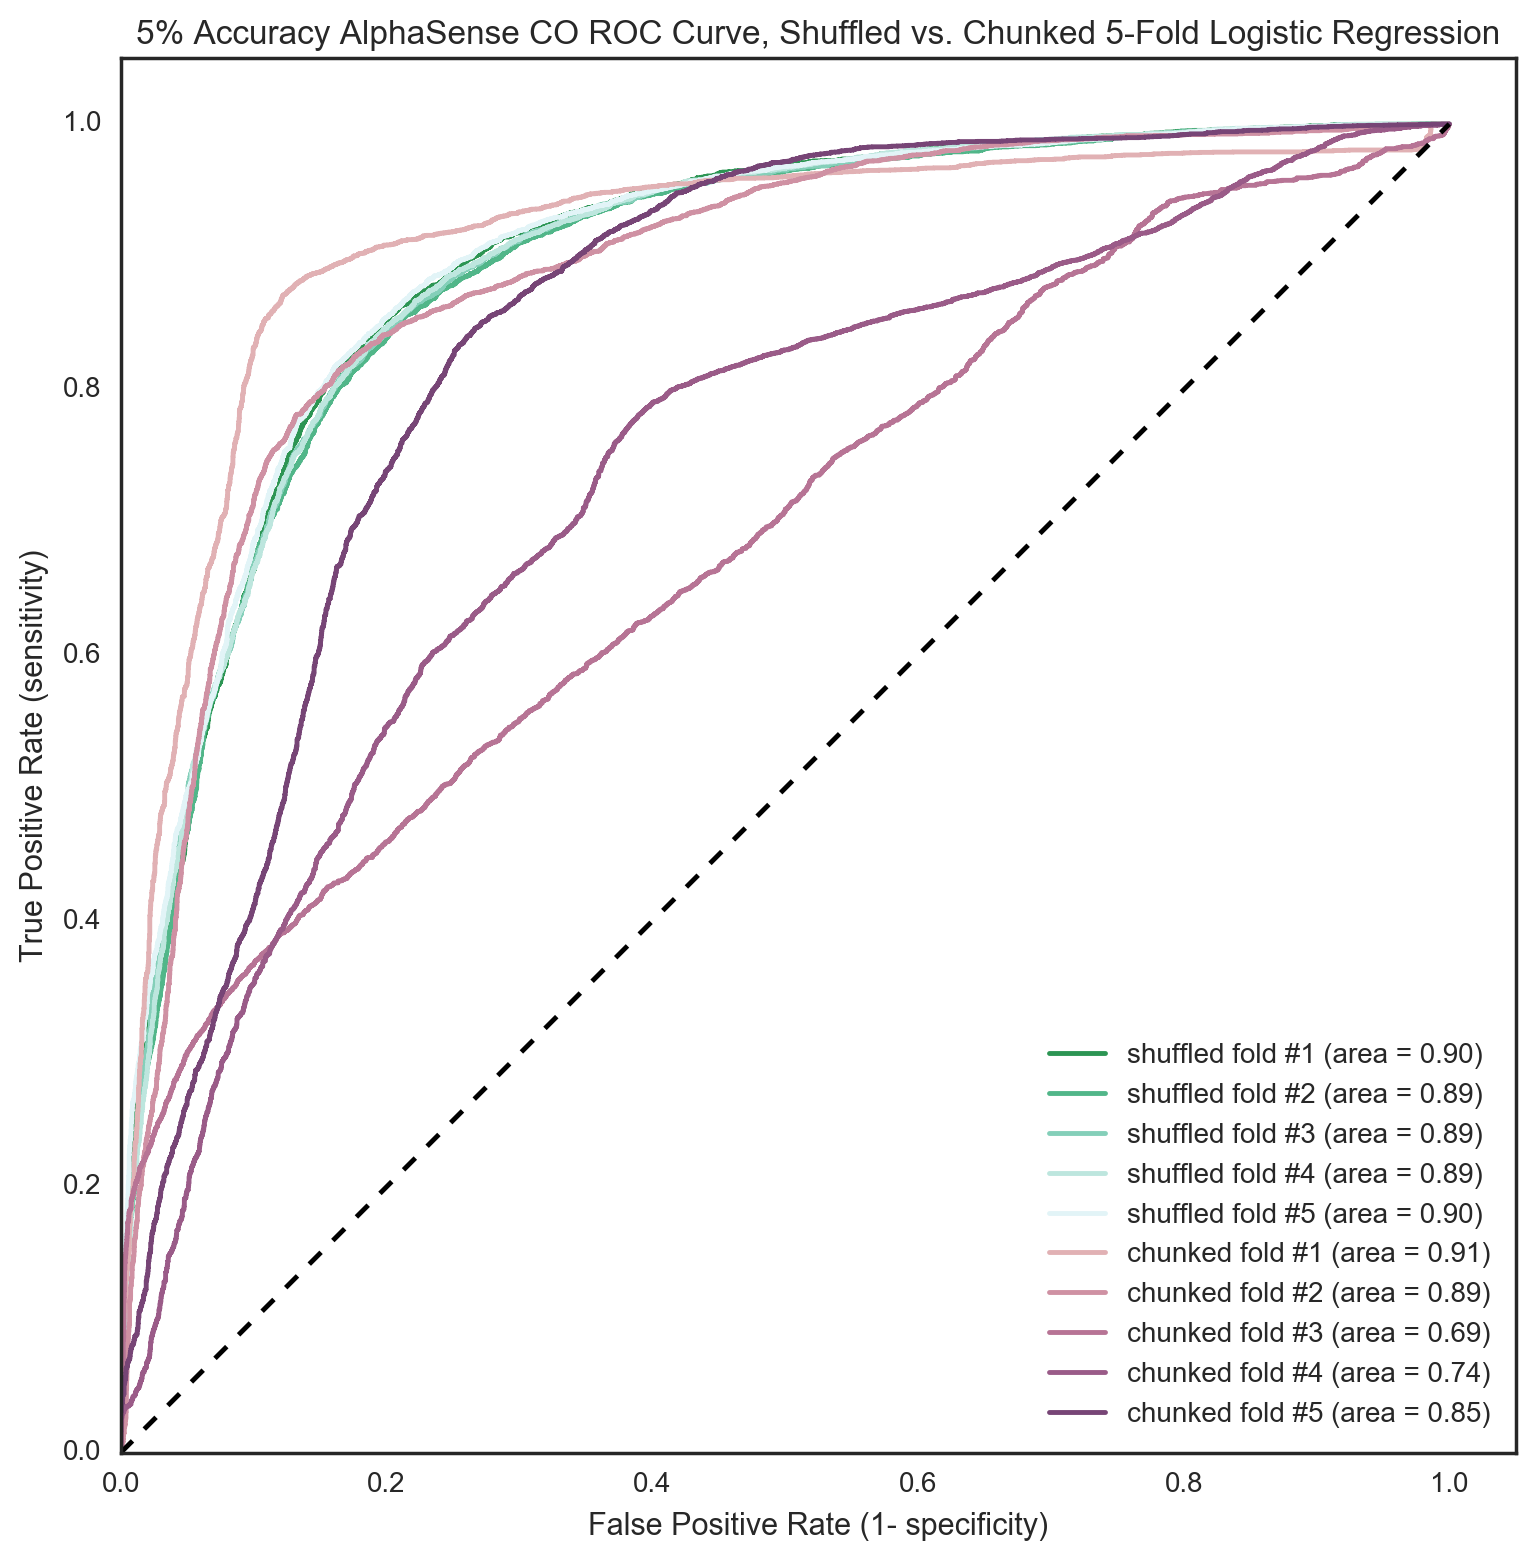
\includegraphics[width=\textwidth]{figs/as1_co_5_roc}               
 	 \caption{AlphaSense CO Sensor #1 ROC Curve}
  	\label{fig:as1_co_5_roc}
\end{figure}


here's text referencing the (Table \ref{tab:as1_co_randomforest_features}).

\begin{table}[H]
\centering
\begin{tabular}{lllllllll}
\\
\\
\toprule
Feature & Importance \\
\midrule
lmse\_calib\_as\_co & 0.0331983839664 \\
avg\_15\_lmse\_calib\_as\_co & 0.0331946346979 \\
avg\_15\_as\_co & 0.0322602817136 \\
as\_co & 0.0310204625161 \\
sck\_temperature & 0.0271023795431 \\
avg\_15\_as\_temperature & 0.0251288063362 \\
Temperature ( C RAW) & 0.024693128613 \\
avg\_60\_forecastio\_temperature_c & 0.0207050630804 \\
forecastio\_temperature\_c & 0.0192957142054 \\
as\_temperature & 0.018952457567 \\
avg\_60\_forecastio\_apparentTemperature & 0.017952895033 \\
alphaTemp & 0.0177934801727 \\
temp\_as\_box\_differential & 0.017581796276 \\
forecastio\_temperature & 0.0159096583245 \\
temp\_sck\_box\_differential & 0.0150463135619 \\
\bottomrule
\end{tabular}
\label{tab:as1_co_randomforest_features}
\caption{Top 15 Features from Random Forest for CO Sensor #1, used in Pruned Logistic Regression}
\end{table}



\begin{figure}[htb]
 	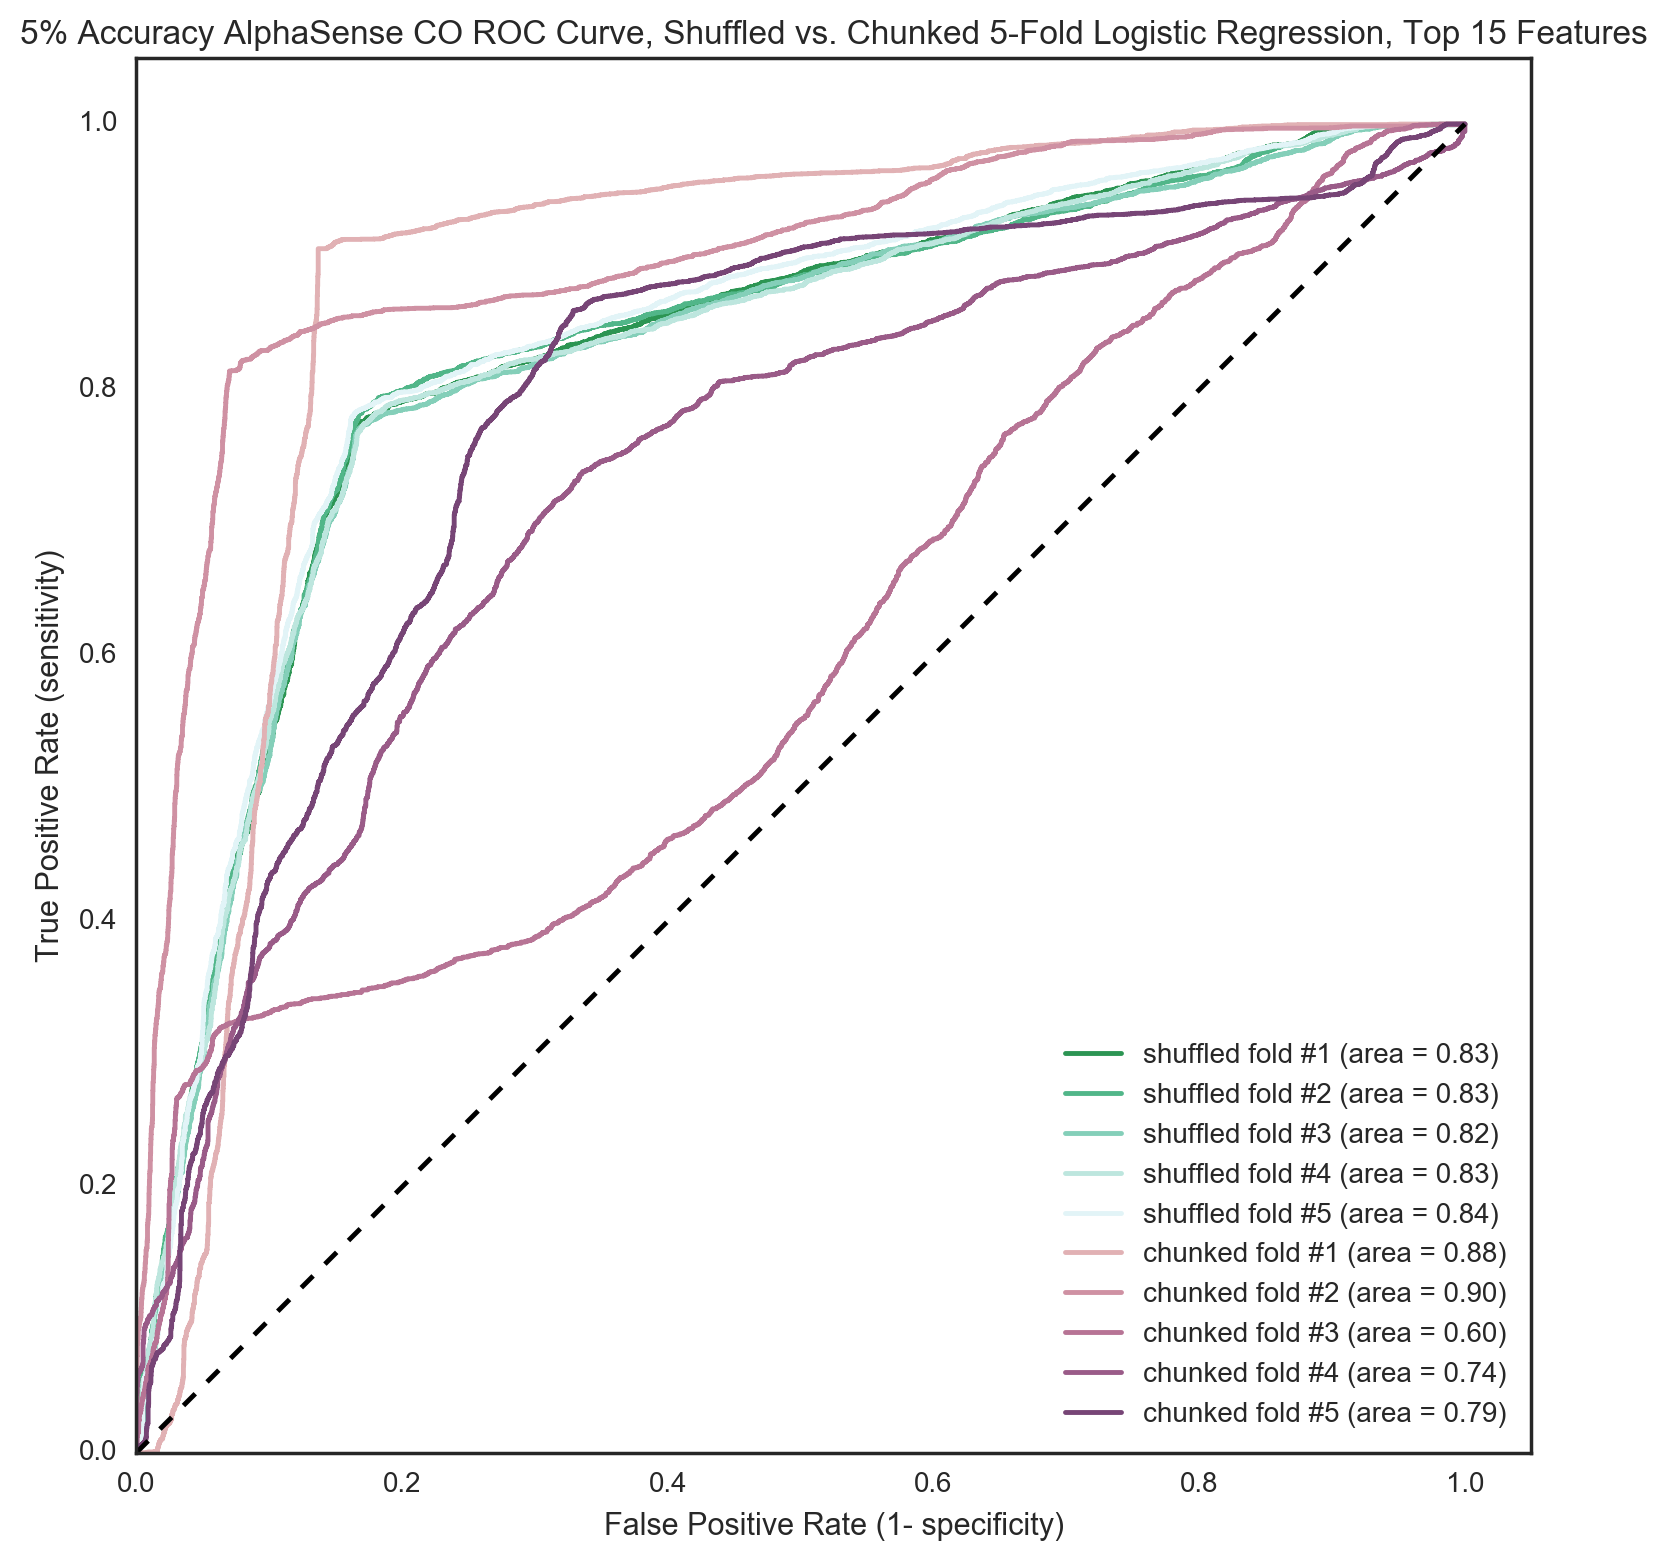
\includegraphics[width=\textwidth]{figs/as1_co_5_roc_pruned_features}               
 	 \caption{AlphaSense CO Sensor #1 ROC Using Top 15 Features}
  	\label{fig:as1_co_5_roc_pruned_features}
\end{figure}

\begin{figure}[htb]
 	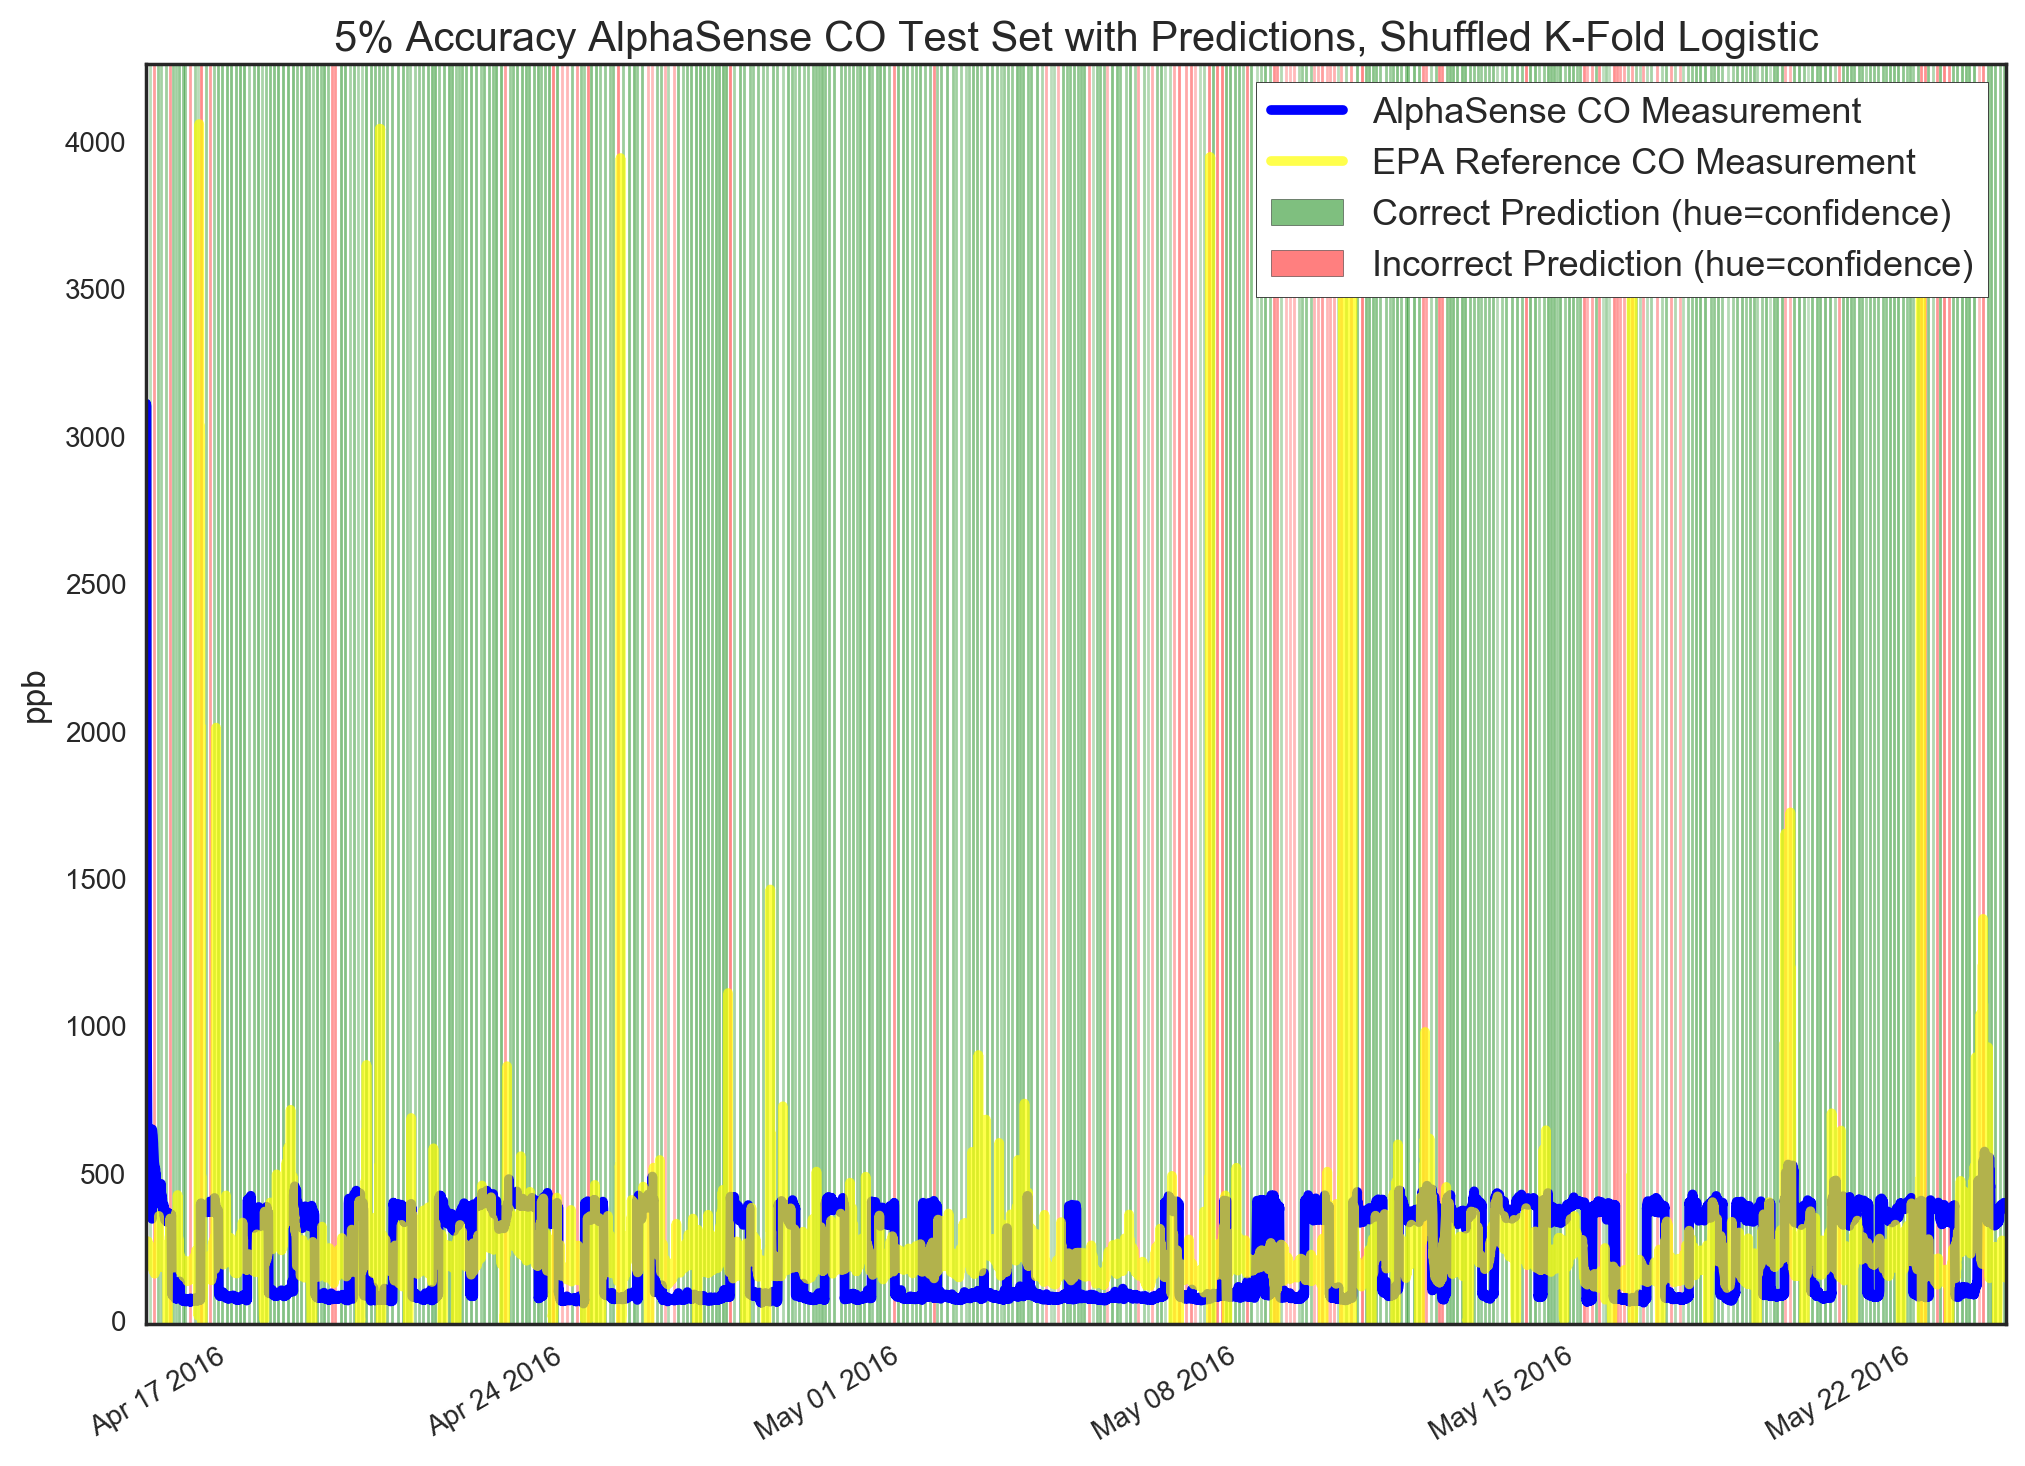
\includegraphics[width=\textwidth]{figs/as1_co_5_logistic_predictions}               
 	 \caption{AlphaSense CO Sensor #1 Prediction Accuracy}
  	\label{fig:as1_co_5_logistic_predictions}
\end{figure}



here's text referencing the (Table \ref{tab:as1_co_top_features}).

\begin{table}[H]
\centering
\begin{tabular}{lllllllll}
\\
\\
\toprule
     & Corr. & Lasso & Lin Reg & RF   & RFE  & Ridge & Stability & Mean \\
\midrule
as\_co                                        & 0.95  & 0.29  & 0          & 1    & 0.64 & 0     & 0.51      & 0.48 \\
lmse\_calib\_as\_co                           & 0.95  & 0     & 0          & 0.68 & 0.65 & 0     & 0.59      & 0.41 \\
avg\_60\_forecastio\_humidity                 & 0.29  & 0     & 0.01       & 0.03 & 1    & 0.73  & 0.59      & 0.38 \\
forecastio\_wind                              & 0     & 0     & 0.05       & 0    & 0.76 & 0.54  & 1         & 0.34 \\
sck\_temperature                              & 0.92  & 0     & 0          & 0.02 & 0.98 & 0     & 0.44      & 0.34 \\
alphaS2\_work                                 & 0     & 1     & 0          & 0.02 & 0.25 & 0.01  & 1         & 0.33 \\
alphaTemp                                     & 0.94  & 0     & 0          & 0    & 0.92 & 0     & 0.48      & 0.33 \\
as\_temperature                               & 0.94  & 0     & 0          & 0    & 0.91 & 0     & 0.46      & 0.33 \\
humidity\_box\_differential                   & 0.14  & 0     & 0.01       & 0.04 & 1    & 0.73  & 0.37      & 0.33 \\
avg\_15\_as\_temperature                      & 0.99  & 0     & 0          & 0.02 & 0.57 & 0.16  & 0.49      & 0.32 \\
avg\_720\_lmse\_scaled\_sharpDust             & 0.02  & 0     & 0          & 0.03 & 0.54 & 1     & 0.68      & 0.32 \\
Temperature ( C RAW)                          & 0.92  & 0.07  & 0          & 0.02 & 0.63 & 0     & 0.45      & 0.3  \\
Solar Panel ( V)                              & 0.14  & 0     & 1          & 0    & 0.95 & 0     & 0         & 0.3  \\
forecastio\_temperature                       & 0.68  & 0.09  & 0          & 0    & 0.87 & 0     & 0.37      & 0.29 \\
avg\_60\_forecastio\_temperature\_c           & 0.7   & 0     & 0          & 0.03 & 0.97 & 0.09  & 0.25      & 0.29 \\
evening                                       & 0.02  & 0     & 0.1        & 0.02 & 0.99 & 0.04  & 0.81      & 0.28 \\
night                                         & 0.18  & 0     & 0.05       & 0    & 1    & 0.11  & 0.59      & 0.28 \\
day                                           & 0.18  & 0     & 0.05       & 0    & 0.96 & 0.11  & 0.6       & 0.27 \\
forecastio\_temperature\_c                    & 0.68  & 0     & 0          & 0    & 0.88 & 0     & 0.31      & 0.27 \\
morning                                       & 0.01  & 0     & 0.1        & 0    & 1    & 0.12  & 0.61      & 0.26 \\
avg\_60\_forecastio\_cloudCover               & 0     & 0     & 0          & 0.04 & 0.48 & 0.29  & 1         & 0.26 \\
forecastio\_humidity                          & 0.28  & 0     & 0          & 0    & 0.55 & 0.26  & 0.69      & 0.25 \\
derivative\_avg\_720\_lmse\_scaled\_sharpDust & 0     & 0     & 0          & 0.01 & 0.61 & 0.15  & 1         & 0.25 \\
hour\_of\_day                                 & 0.02  & 0.41  & 0          & 0.01 & 0.22 & 0.01  & 1         & 0.24\\
\bottomrule
\end{tabular}
\label{tab:as1_co_top_features}
\caption{Top Features for Predicting AlphaSense CO Sensor #1}
\end{table}




parameters = {'C':[0.001, 0.1, 10, 1000], 'penalty':('L1', 'L2') }

===== best ROC_AUC score 0.904107344914

===== best params {'penalty': 'L1', 'C': 1000}

\begin{table}[H]
\centering
\begin{tabular}{|c|c|c|c|c|}
\toprule
\multicolumn{5}{|c|}{Error Rates for CO Sensor #2 with Logistic Regression} \\
&\multicolumn{2}{|c|}{all features} & \multicolumn{2}{|c|}{top 15 features} \\
&shuffled & chunked & shuffled & chunked \\
avg & 0.14 & 0.20 & 0.16 & 0.17 \\
min & 0.13 & 0.10 & 0.15 & 0.11 \\
max & 0.14 & 0.28 & 0.16 & 0.22 \\
\bottomrule
\end{tabular}
\label{tab:as2_co_error_rates}
\caption{Error Rates for Predicting CO Sensor #2 Accuracy with Logistic Regression}
\end{table}


\begin{table}[H]
\centering
\offinterlineskip
\hspace*{-5cm}\raisebox{-3.5cm}[0pt][0pt]{\rotatebox[origin=c]{90}{\parbox[c][0pt][c]{3cm}{\textbf{Actual Values}\\[20pt]}}}\par
\hspace*{1cm}\MyHBox[\dimexpr5.1cm+6\fboxsep\relax]{Predicted Values}\par
\hspace*{1cm}\MyHBox{0}\MyHBox{1}\par
\MyTBox{0}{1326.2}{623.0}
\MyTBox{1}{200.4}{3880.4}
}
\label{tab:as2_co_confusion}
\caption{Average AlphaSense CO Sensor #2 Confusion Matrix w/Shuffled K-Fold}
\end{table}


\begin{figure}[htb]
 	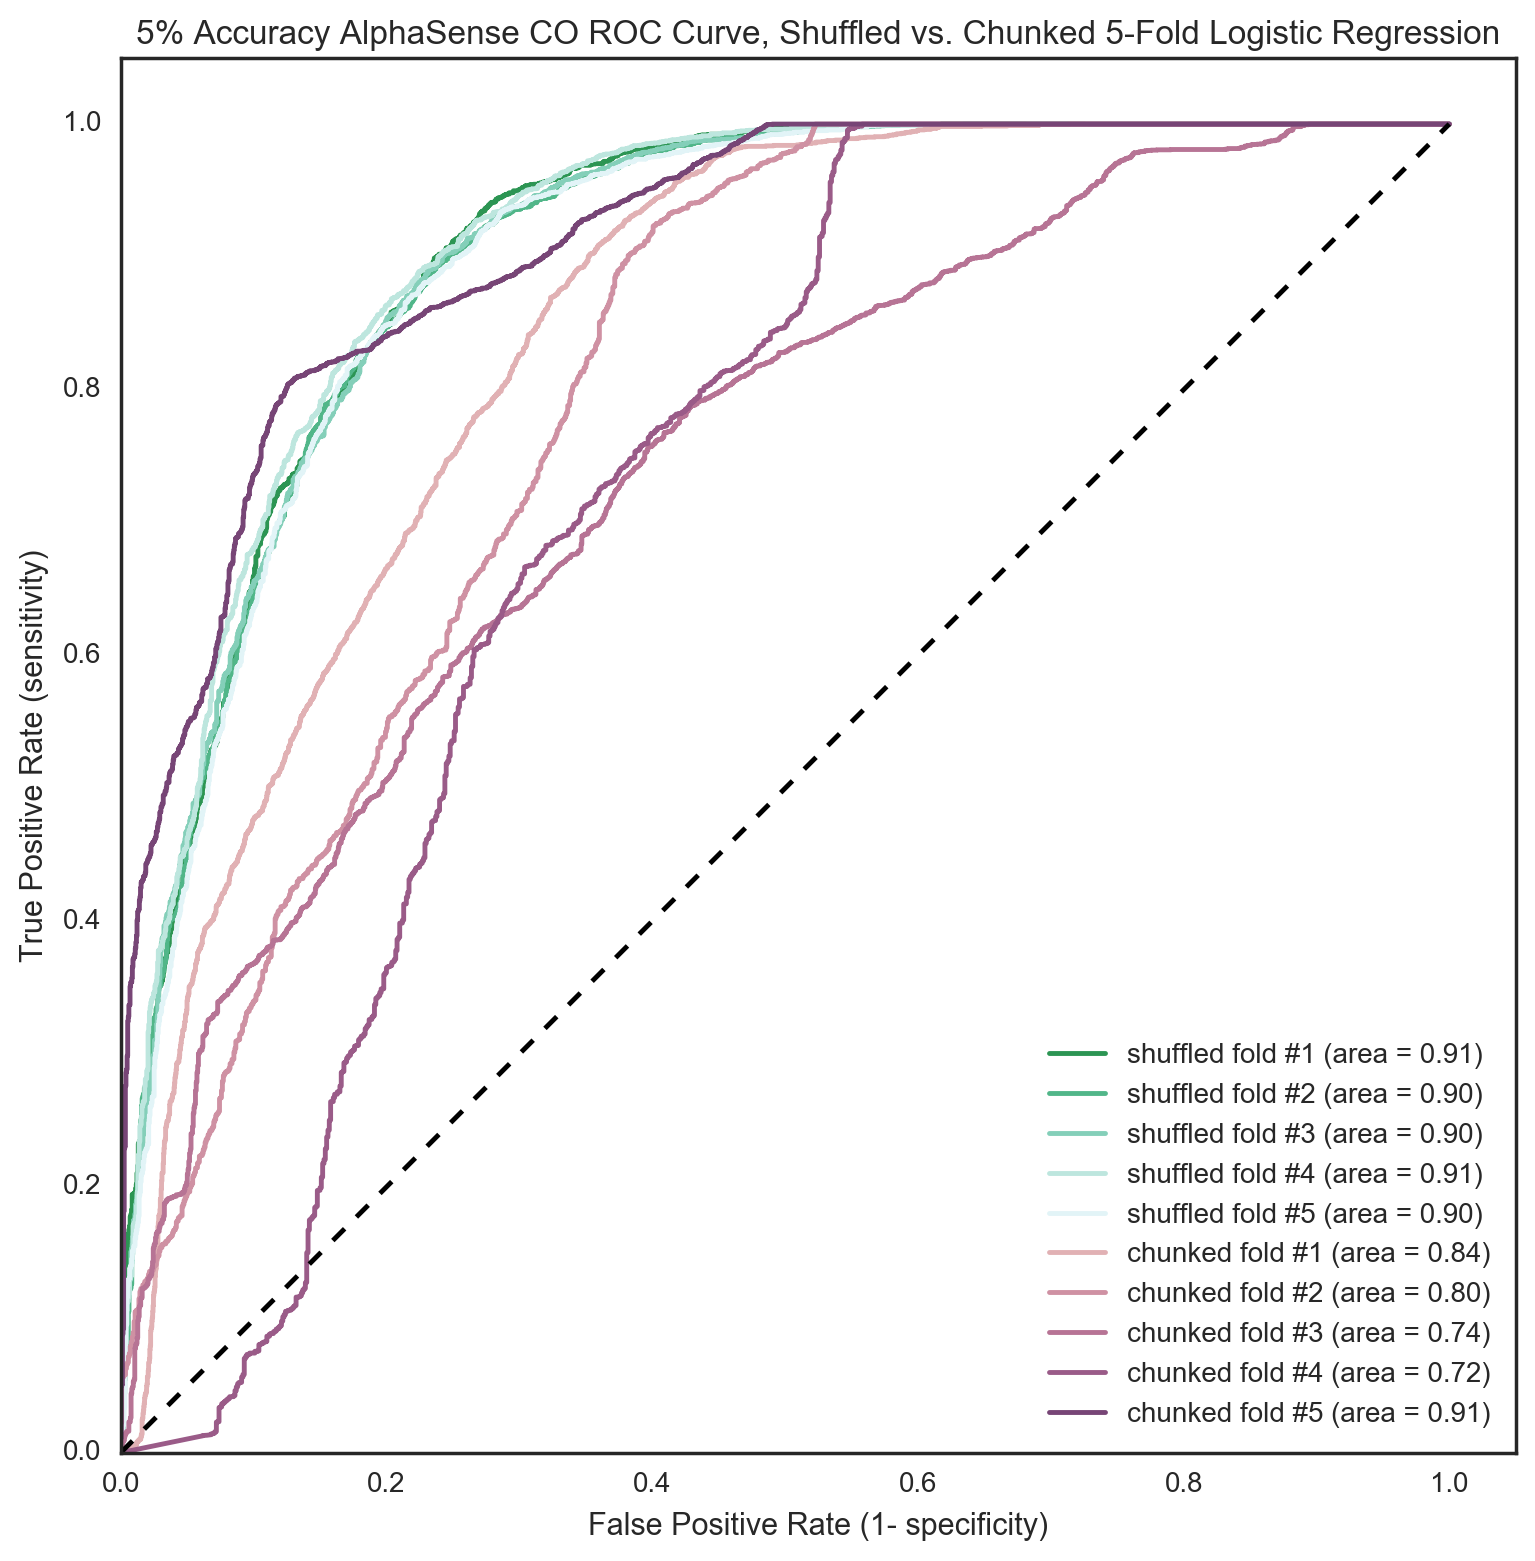
\includegraphics[width=\textwidth]{figs/as2_co_5_roc}               
 	 \caption{AlphaSense CO Sensor #2 ROC Curve}
  	\label{fig:as2_co_5_roc}
\end{figure}



here's text referencing the (Table \ref{tab:as2_o3_randomforest_features}).

\begin{table}[H]
\centering
\begin{tabular}{lllllllll}
\\
\\
\toprule
Feature & Importance \\
\midrule
lmse\_calib\_as\_co & 0.0518584805682 \\
avg\_15\_lmse\_calib\_as\_co & 0.0404238890793 \\
avg\_720\_bkcarbon & 0.0222537733125 \\
avg\_60\_bkcarbon & 0.0216045744972 \\
avg\_1440\_bkcarbon & 0.0198813295966 \\
as\_o3 & 0.0198510401658 \\
lmse\_as\_no2 & 0.0197364055605 \\
avg\_10\_as\_o3 & 0.0196965727088 \\
bkcarbon & 0.0194862747741 \\
as\_no2 & 0.0192353467551 \\
avg\_15\_lmse\_as\_no2 & 0.0180978893662 \\
lmse\_avg\_15\_as\_no2 & 0.0172526534474 \\
avg\_15\_as\_no2 & 0.0162905415767 \\
avg\_15\_as\_co & 0.0158810645781 \\
as\_co & 0.0158442759727 \\
\bottomrule
\end{tabular}
\label{tab:as2_co_randomforest_features}
\caption{Top 15 Features from Random Forest for CO Sensor #2, used in Pruned Logistic Regression}
\end{table}


\begin{figure}[htb]
 	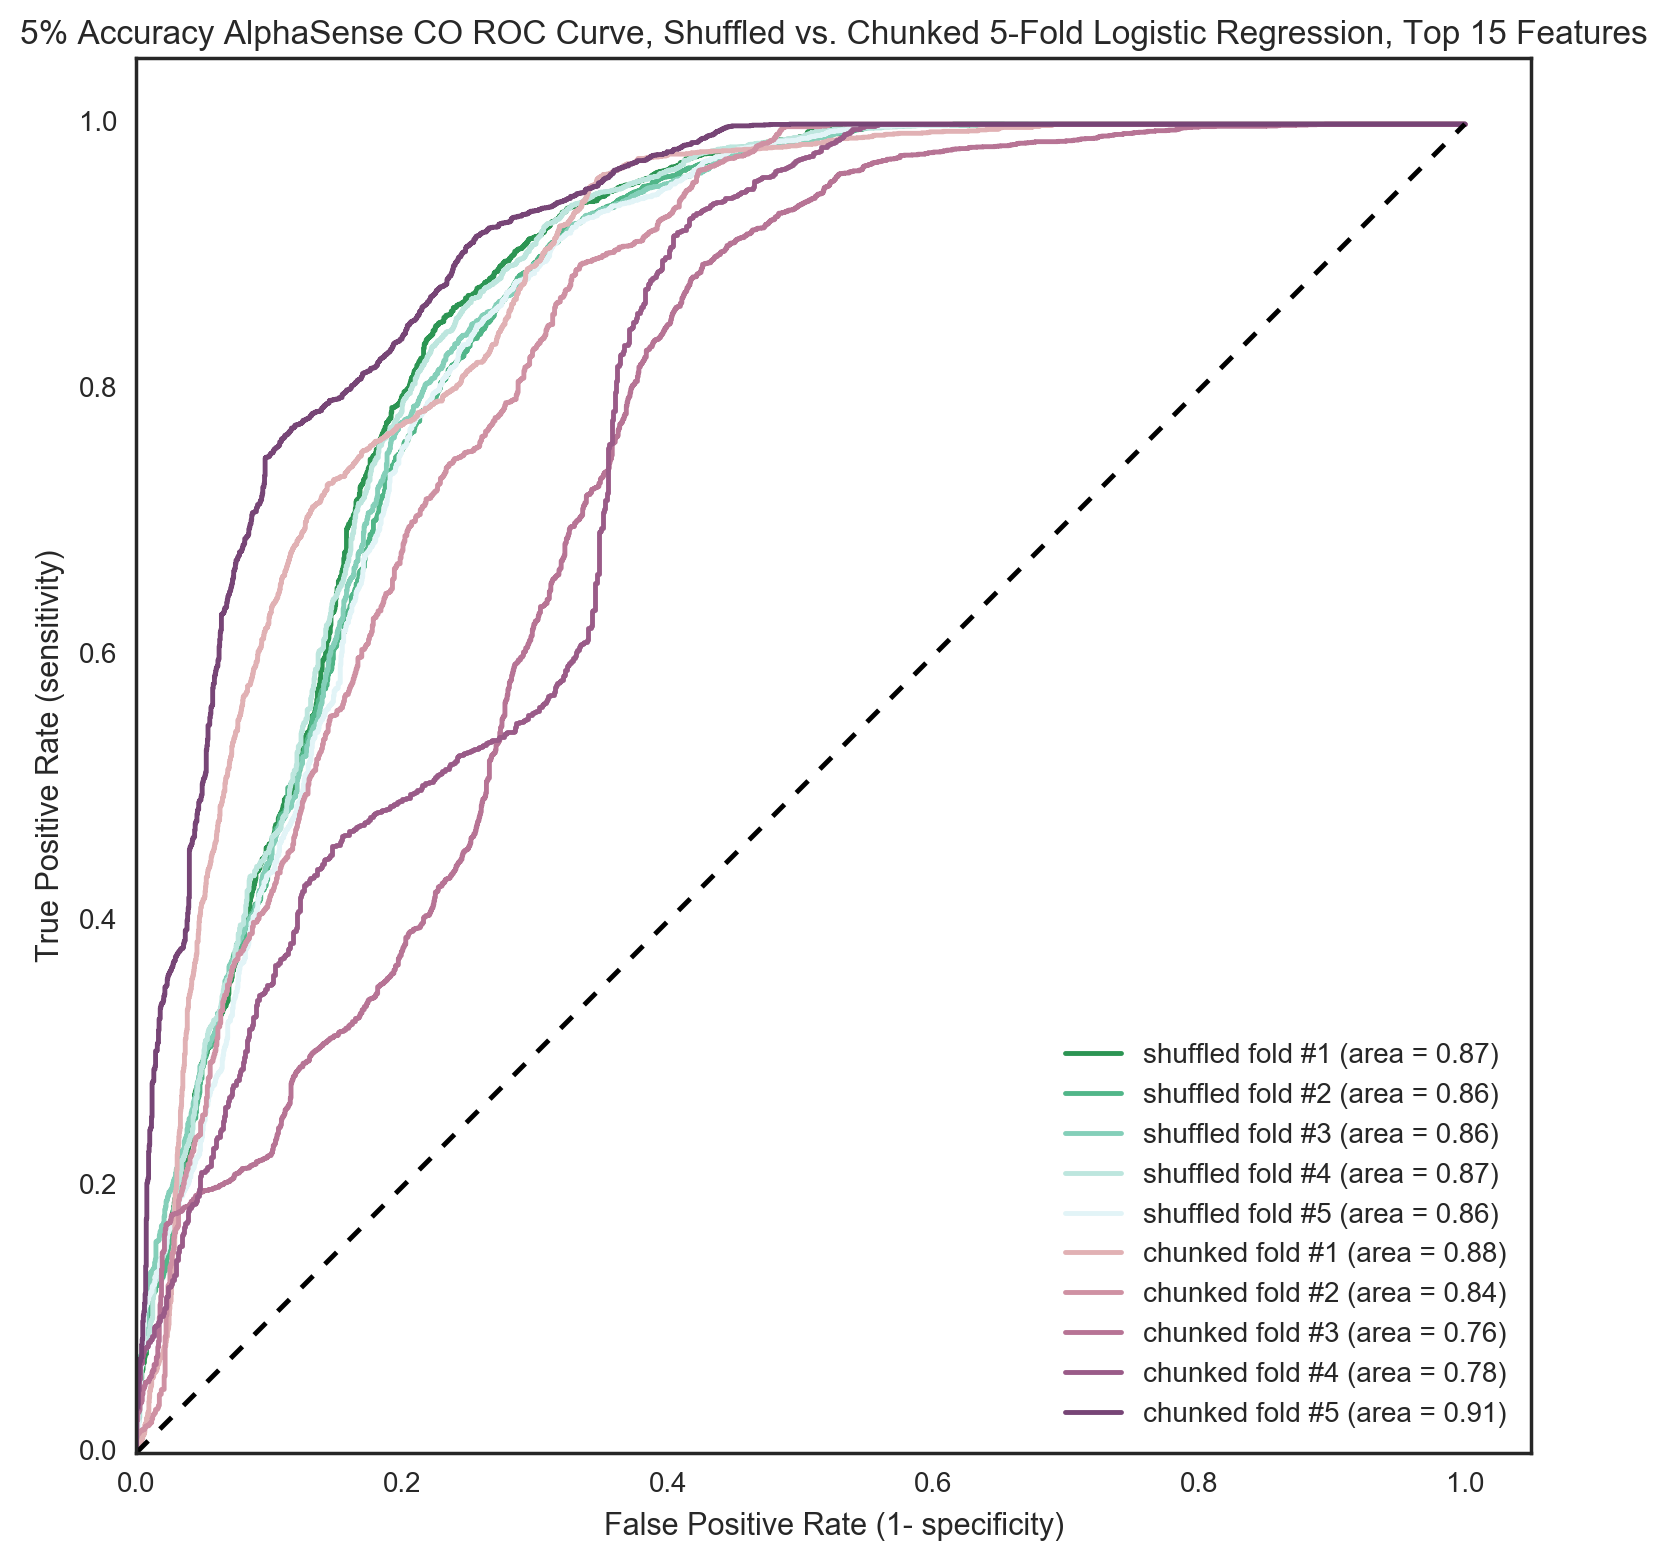
\includegraphics[width=\textwidth]{figs/as2_co_5_roc_pruned_features}               
 	 \caption{AlphaSense CO Sensor #2 ROC Using Top 15 Features}
  	\label{fig:as2_o3_7p5_roc_pruned_features}
\end{figure}

\begin{figure}[htb]
 	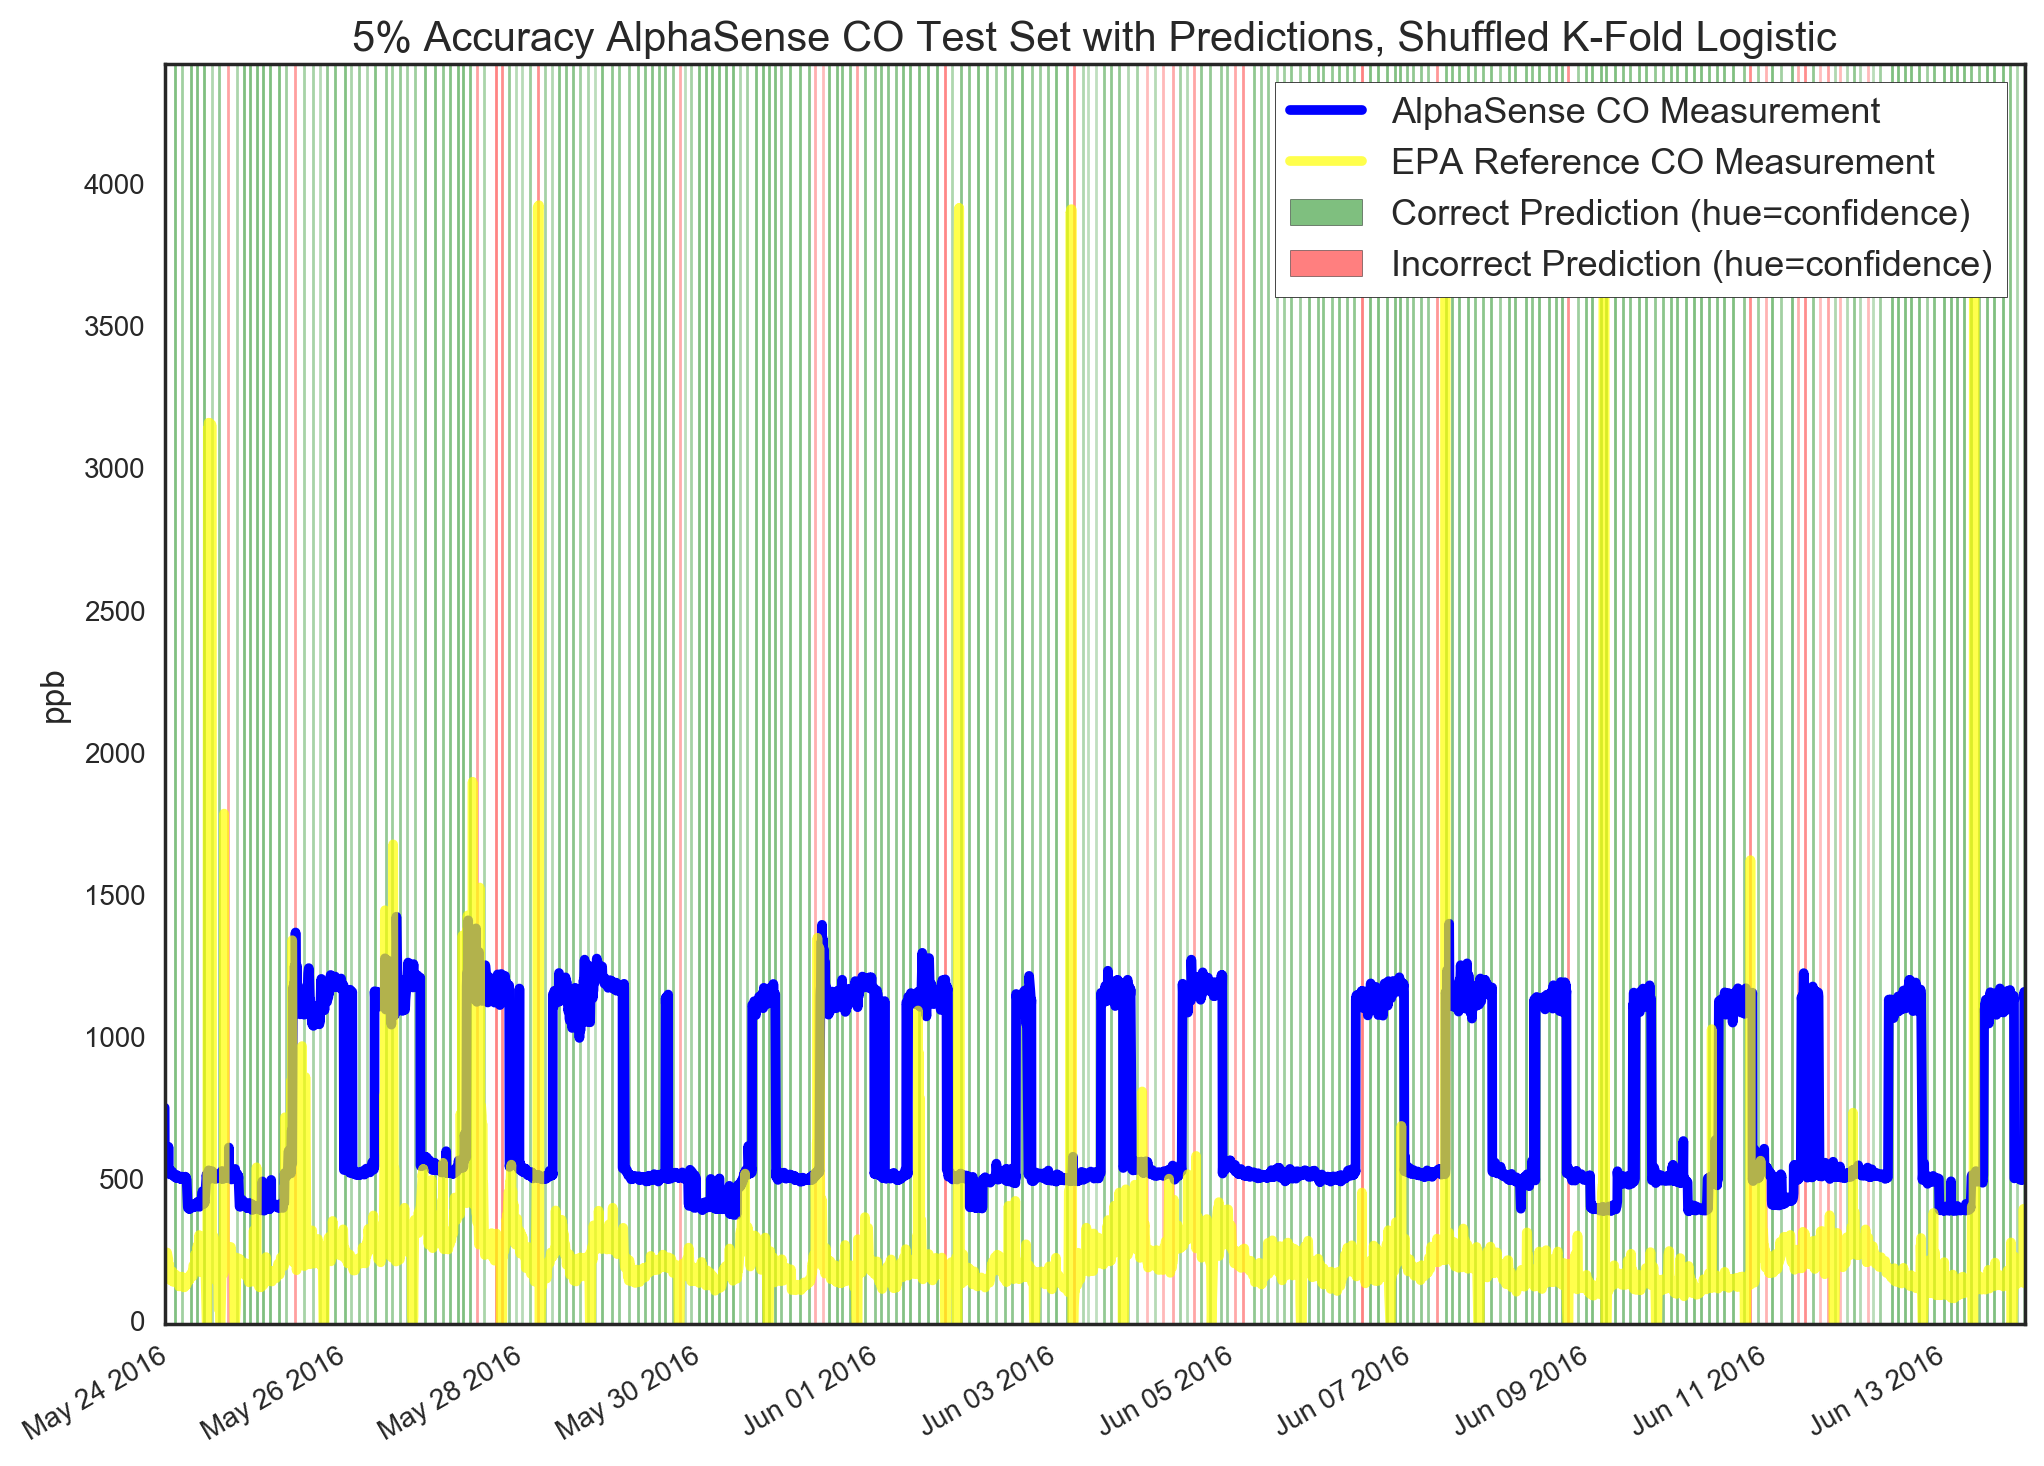
\includegraphics[width=\textwidth]{figs/as2_co_5_logistic_predictions}               
 	 \caption{AlphaSense CO Sensor #2 Prediction Accuracy}
  	\label{fig:as2_co_5_logistic_predictions}
\end{figure}


here's text referencing the (Table \ref{tab:as2_co_top_features}).

\begin{table}[H]
\centering
\begin{tabular}{lllllllll}
\\
\\
\toprule
     & Corr. & Lasso & Lin Reg & RF   & RFE  & Ridge & Stability & Mean \\
\midrule
lmse\_calib\_as\_co                            & 1     & 0.1   & 0          & 1    & 0.18 & 0     & 1         & 0.47 \\
evening                                        & 0     & 0     & 0.01       & 0.01 & 0.96 & 0.04  & 0.99      & 0.29 \\
avg\_60\_forecastio\_windSpeed                 & 0.3   & 1     & 0          & 0.15 & 0.06 & 0     & 0.55      & 0.29 \\
Solar Panel ( V)                               & 0.11  & 0     & 1          & 0    & 0.86 & 0     & 0         & 0.28 \\
forecastio\_windSpeed                          & 0.27  & 0.62  & 0          & 0.02 & 0.29 & 0.01  & 0.72      & 0.28 \\
sck\_humidity\_saturated                       & 0.05  & 0     & 0          & 0    & 0.59 & 1     & 0.33      & 0.28 \\
avg\_15\_as\_no2                               & 0.4   & 0.29  & 0          & 0.01 & 0.73 & 0     & 0.36      & 0.26 \\
forecastio\_fog                                & 0.11  & 0     & 0.71       & 0    & 0.94 & 0     & 0         & 0.25 \\
as\_o3                                         & 0.41  & 0.08  & 0          & 0.01 & 0.72 & 0     & 0.5       & 0.25 \\
derivative\_avg\_1440\_lmse\_scaled\_sharpDust & 0.14  & 0     & 0          & 0.01 & 0.6  & 0.03  & 0.99      & 0.25 \\
as\_no2                                        & 0.41  & 0     & 0          & 0    & 0.71 & 0.01  & 0.53      & 0.24 \\
lmse\_as\_no2                                  & 0.41  & 0     & 0          & 0    & 0.73 & 0     & 0.48      & 0.23 \\
lmse\_avg\_15\_as\_no2                         & 0.4   & 0     & 0.01       & 0.01 & 0.81 & 0     & 0.41      & 0.23 \\
bkcarbon                                       & 0.05  & 0     & 0          & 0.13 & 0.5  & 0.1   & 0.81      & 0.23 \\
avg\_15\_derivative\_sck\_temperature          & 0     & 0     & 0          & 0.01 & 0.57 & 0.41  & 0.53      & 0.22 \\
daily\_avg\_forecastio\_temperature            & 0.22  & 0     & 0          & 0.03 & 0.45 & 0.1   & 0.71      & 0.22 \\
avg\_15\_lmse\_as\_no2                         & 0.4   & 0     & 0.01       & 0.01 & 0.82 & 0     & 0.3       & 0.22 \\
derivative\_avg\_360\_lmse\_as\_no2            & 0     & 0     & 0          & 0.02 & 0.59 & 0.31  & 0.62      & 0.22 \\
avg\_60\_bkcarbon                              & 0.06  & 0     & 0          & 0.07 & 0.55 & 0.15  & 0.73      & 0.22 \\
afternoon                                      & 0.13  & 0     & 0.01       & 0    & 0.97 & 0.06  & 0.31      & 0.21 \\
avg\_720\_bkcarbon                             & 0.02  & 0     & 0          & 0.18 & 0.53 & 0.06  & 0.69      & 0.21 \\
alphaS2\_work                                  & 0.02  & 0.61  & 0          & 0.03 & 0.23 & 0.02  & 0.49      & 0.2  \\
avg\_60\_as\_no2                               & 0.39  & 0.01  & 0          & 0.02 & 0.99 & 0     & 0         & 0.2  \\
avg\_15\_lmse\_calib\_as\_co                   & 0.94  & 0     & 0          & 0.05 & 0.05 & 0     & 0.35      & 0.2 \\
\bottomrule
\end{tabular}
\label{tab:as2_co_top_features}
\caption{Top Features for Predicting AlphaSense CO Sensor #2}
\end{table}